\documentclass[aps,pra,twocolumn,10pt,amsmath,amssymb,floatfix]{revtex4-2}

\usepackage[T1]{fontenc}
\usepackage{amsthm,mathtools}
\usepackage{booktabs}
\usepackage{array}
\usepackage{graphicx}
\usepackage{xcolor}
\usepackage{microtype}
\usepackage{enumitem}
\usepackage[colorlinks=true,linkcolor=blue!55!black,citecolor=blue!55!black,urlcolor=blue!55!black]{hyperref}

\theoremstyle{plain}
\newtheorem{theorem}{Theorem}
\newtheorem{proposition}[theorem]{Proposition}
\newtheorem{lemma}[theorem]{Lemma}
\newtheorem{corollary}[theorem]{Corollary}

\theoremstyle{definition}
\newtheorem{definition}[theorem]{Definition}
\newtheorem{remark}[theorem]{Remark}

\newcommand{\dd}{\mathrm{d}}
\newcommand{\ii}{\mathrm{i}}
\newcommand{\ee}{\mathrm{e}}
\newcommand{\Tr}{\operatorname{Tr}}
\newcommand{\sgn}{\operatorname{sgn}}
\newcommand{\NBLP}{\mathcal{N}_{\mathrm{BLP}}}
\newcommand{\IRHP}{\mathcal{I}_{\mathrm{RHP}}}
\newcommand{\IRHPreg}{\mathcal{I}_{\mathrm{RHP}}^{(\epsilon)}}
\newcommand{\mupole}{\mu_{\mathrm{pole}}}
\newcommand{\mucrit}{\mu_{\mathrm{crit}}}
\newcommand{\muzero}{\mu_{\mathrm{zero}}}
\newcommand{\mustar}{\mu_*}
\newcommand{\leanid}[1]{{\footnotesize\ttfamily\def\_{\textunderscore\penalty0\hspace{0pt}}#1}}

\begin{document}
\setlength{\emergencystretch}{3em}

\title{Exact Analytic Phase Boundary Between Complete Monotonicity, Completely Positive Divisibility, and Information Backflow in Time-Subordinated Open Quantum Dynamics}

\author{Mehardeep Singh}
\email{mehardeep.sim@gmail.com}
\affiliation{Sri Chaitanya Educational Institutions}

\date{}

\begin{abstract}
We determine the exact phase structure separating complete monotonicity (CM), completely positive (CP) divisibility, P-divisibility, Spohn relative-entropy monotonicity, and global complete positivity in open quantum dynamics governed by inverse $\mu$-stable time subordination ($\mu \in (0,1]$, dimensionless switching rate $g > 0$). Starting from a bipartite Markovian random-telegraph-noise semigroup on $\mathbb{C}^2_S \otimes \mathbb{C}^2_M$, operational-time subordination yields an exact unital pure-dephasing channel whose coherence propagator has Laplace transform $\tilde{G}_{\mu,g}(s) = s^{\mu-1}(s^\mu + 2g)/(s^{2\mu} + 2g s^\mu + 1)$, guaranteeing global complete positivity ($|G_{\mu,g}(t)| \le 1$) and universal Helstrom optimality of antipodal equatorial states for the Breuer--Laine--Piilo (BLP) trace-distance measure $\NBLP(\mu,g)$. Deriving the exact Hankel branch-cut spectral density $K_{\mu,g}(r)$, we prove that $G_{\mu,g}(t)$ is completely monotonic on $(0,\infty)$ if and only if $\mu \in (0,1/2]$ for every $g > 0$. Using a general Single-Sign-Change Laplace Positivity Theorem, we prove that $\dot{G}_{\mu,g}(t) < 0$ strictly for all $t > 0$---establishing strict CP-divisibility and $\NBLP = \IRHP = 0$---across the entire pole-free wedge comprising all $\mu \in (0,1]$ for $g \ge 1$ and $\mu \in (0,\mupole(g)]$ with $\mupole(g) := 1 - \arccos(g)/\pi$ for $g \in (0,1)$. Resolving the Cauchy competition between principal-sheet pole residues and the negative branch-cut integral ($\dot{G}_{\mu,g} = \dot{G}_{\mathrm{pole}} + \dot{G}_{\mathrm{cut}}$) via 55-digit 2D Newton root finding cross-checked at 70 working digits to $2.23 \times 10^{-72}$ against two-parameter Mittag-Leffler series, we demonstrate a strict \emph{pole-suppressed CP-divisible buffer} $\mucrit(g) > \mupole(g)$ across all $g \in (0,1)$ (peaking at $\mucrit - \mupole = 0.164606$ for $g=0.75$), derive its super-exponential asymptotic law $1 - \mucrit(g) \sim [\pi^2/(2\ee(1-g^2))]\exp(-\pi g/\sqrt{1-g^2})$ as $g \to 1^-$, show continuous matching onto the known Markovian ($\mu=1$) law $\NBLP(1,g) = (\exp(\pi g/\sqrt{1-g^2}) - 1)^{-1}\mathbf{1}_{g<1}$, and prove that backflow and zero crossings ($G_{\mu,g}(t)=0$) occur in at most finitely many intervals whenever $\mu < 1$. Beyond pure dephasing, we combine Pollard log-convexity with a triangle-inequality criterion to show that inverse $\mu$-stable subordination of Markovian Pauli semigroups preserves CP-divisibility on the symmetric transverse ray up to the exact 55-digit threshold $\mustar = 0.9260578001565031$ yet breaks CP-divisibility above $\mustar$ while remaining strictly P-divisible ($\NBLP = 0$) and componentwise completely monotonic---demonstrating that multi-axis componentwise CM does not imply CP-divisibility---and constructively separating the strict six-level hierarchy $\mathrm{SG} \subsetneq \mathrm{CM}_{\mathrm{deph}} \subsetneq \mathrm{CP\text{-}Div} \subsetneq \mathrm{P\text{-}Div} \subsetneq \mathrm{Spohn} \subsetneq \mathrm{CPTP}$. Exact diagonalization of $N=1000$-mode unitary Friedrichs--Lee baths sharpens the distinction between operational-time subordination and microscopic Volterra $E_{2-\mu}$ memory kernels. Twenty-eight headline algebraic, integral-positivity, and $4\times 4$ Choi theorems (within 150 public theorems, 14/28 axiom-free) are machine-checked without external axioms or \texttt{sorry} in pure Lean~4.16.0.
\end{abstract}

\maketitle

%==============================================================================
\section{Introduction}
%==============================================================================

Understanding when non-Markovian open quantum evolutions transition between memoryless semigroups, divisible evolutions, and physical information backflow lies at the heart of quantum master-equation theory~\cite{Breuer2009PRL,Laine2010PRA,Rivas2010PRL,Chruscinski2011PRA,Rivas2014RPP,Breuer2016RMP}. Two conceptually distinct structural notions coexist in the literature: \emph{complete positivity (CP) divisibility}~\cite{Rivas2010PRL,Hall2014PRA,Chruscinski2014PRL,Filippov2017PRA}, which requires every intermediate propagator $\Lambda_{t,s} = \Phi_t \circ \Phi_s^{-1}$ ($t \ge s \ge 0$) to be completely positive (equivalently non-negative canonical Gorini--Kossakowski--Sudarshan--Lindblad (GKSL) rates $\gamma_k(t) \ge 0$~\cite{Lindblad1976,Gorini1976JMP}), and \emph{P-divisibility}~\cite{Chruscinski2014PRL,Wissmann2015PRA,Bae2016PRL}, which requires every $\Lambda_{t,s}$ to be positive and trace-preserving (equivalent for invertible maps to monotonicity of all biased Helstrom operators $p\rho_1 - (1-p)\rho_2$, coinciding with unbiased trace-distance contractivity on unital qubit channels and strictly implying it on non-unital channels). Unbiased information backflow is quantified by the Breuer--Laine--Piilo (BLP) trace-distance functional~\cite{Breuer2009PRL,Laine2010PRA}
\begin{equation}
\NBLP(\Phi) := \max_{\rho_1(0),\,\rho_2(0)} \int_{\sigma_{\mathrm{BLP}}>0} \sigma_{\mathrm{BLP}}\big(t;\rho_1(0),\rho_2(0)\big)\,\dd t,
\end{equation}
where $\sigma_{\mathrm{BLP}}(t;\rho_1,\rho_2) := \frac{\dd}{\dd t} D_{\mathrm{tr}}\big(\Phi_t(\rho_1),\Phi_t(\rho_2)\big)$ and $D_{\mathrm{tr}}(\rho,\sigma) = \frac{1}{2}\Tr|\rho - \sigma|$. While a time-homogeneous GKSL semigroup ($\Lambda_t = \ee^{t\mathcal{L}}$) satisfies complete monotonicity, CP-divisibility, P-divisibility, and Spohn's relative-entropy monotonicity theorem~\cite{Spohn1978JMP} simultaneously, memory-kernel, semi-Markov, random-unitary, and time-subordinated master equations generically fracture these equivalences~\cite{Budini2004PRA,Daffer2004PRA,Shabani2005PRA,Breuer2008PRL,Breuer2009PRE,Vacchini2013PRA,Addis2014PRA,Hall2014PRA,Chruscinski2015PRA,Chruscinski2016PRA,Vacchini2016PRL,Megier2017SciRep,Filippov2017PRA}.

In classical and quantum stochastic processes, \emph{subordination} enters through three mathematically inequivalent mechanisms that must be carefully distinguished:
\begin{enumerate}[leftmargin=1.4em,itemsep=2pt]
\item \textbf{Bochner--Phillips convolution semigroup subordination~\cite{Bochner1949PNAS,Bochner1955Book,Phillips1952PJM}:} Randomizing the clock of a strongly continuous contraction semigroup $T(\tau)=\ee^{\tau\mathcal{L}}$ via a Bernstein function $\psi$ preserves the semigroup property, $\int_0^\infty T(\tau)\,q_t(\dd\tau) = \ee^{-t\psi(-\mathcal{L})}$, because the L\'evy transition kernels $q_t$ form a convolution semigroup ($q_{t+s} = q_t * q_s$). Such maps are \emph{always} time-homogeneous Markovian GKSL semigroups with zero non-Markovianity.
\item \textbf{Operational-time inverse subordination:} Following Refs.~\cite{Sokolov2001PRE,Sokolov2002PRE,Meerschaert2004JAP,Budini2004PRA,Breuer2008PRL,Breuer2009PRE,Vacchini2013PRA}, evaluating a contraction family $T(\tau)$ along the inverse $\mu$-stable hitting-time process $\tau = S_\mu^{-1}(t)$ ($\mu \in (0,1]$) yields $\Phi_\mu(t) = \int_0^\infty T(\tau)\,p_\mu(\tau,t)\,\dd\tau$, whose Laplace transform reads $\tilde{\Phi}_\mu(s) = s^{\mu-1}\tilde{T}(s^\mu)$; for a Markovian semigroup $T(\tau) = \ee^{\tau\mathcal{L}}$, this reduces to $s^{\mu-1}(s^\mu - \mathcal{L})^{-1}$ (solving the Caputo fractional generator equation ${}^C D_t^\mu \Phi_\mu(t) = \mathcal{L}\Phi_\mu(t)$) rather than $(s^\mu - \mathcal{L})^{-1}$, while extending directly to arbitrary non-Markovian dynamical families $T(\tau)$. Because $p_\mu(\tau,t)$ is \emph{not} a convolution semigroup in $t$, $\Phi_\mu(t)$ immediately departs from the Markovian semigroup manifold.
\item \textbf{Microscopic unitary Hamiltonian baths~\cite{Friedrichs1948CPAM,Lee1954PR,Garraway1997PRA}:} Exact unitary evolution $H = \omega_0|e\rangle\langle e| + \sum_k \omega_k b_k^\dagger b_k + \sum_k g_k(|e\rangle\langle g|b_k + \mathrm{H.c.})$ with spectral density $J(\omega)$ obeys a linear Volterra integro-differential memory kernel $\dot{c}(t) + \ii\omega_0 c(t) = -\int_0^t K_{\mathrm{FL}}(t-\tau)c(\tau)\,\dd\tau$. For singular low-frequency spectra $J(\omega)\propto\omega^{\mu-1}\ee^{-\omega/\omega_c}$, the Laplace self-energy behaves as $\Sigma(s)\sim c\,s^{\mu-1}$ rather than a time-change scaling $s^\mu$, producing $E_{2-\mu}$ oscillatory Volterra dynamics and bound states rather than inverse-stable subordination.
\end{enumerate}

The purpose of this paper is to solve completely the analytic phase boundary and divisibility hierarchy of inverse $\mu$-stable time-subordinated random-telegraph / damped Jaynes--Cummings coherence dynamics:
\begin{equation}
\label{eq:G_laplace}
\tilde{G}_{\mu,g}(s) = \frac{s^{\mu-1}(s^\mu + 2g)}{s^{2\mu} + 2g s^\mu + 1}, \qquad g > 0,\quad \mu \in (0,1].
\end{equation}
Here $g$ is the dimensionless telegraph switching rate (or cavity damping-to-coupling ratio in the resonant Jaynes--Cummings equivalence~\cite{Daffer2004PRA,Addis2014PRA}). Equation~\eqref{eq:G_laplace} exhibits a rich multi-regime phase structure. Inspection of the complex conjugate poles of $(s^{2\mu}+2gs^\mu+1)^{-1}$ on the principal Riemann sheet $|\arg s| < \pi$ identifies a closed-form pole-entry threshold $\mupole(g) := 1 - \arccos(g)/\pi$ for $g \in (0,1)$, while for $g \ge 1$ poles never leave the negative real branch cut. Whether information backflow ($\dot{G}_{\mu,g}(t) > 0$) coincides with $\mupole(g)$, whether a finite branch-cut stabilization window separates $\mupole(g)$ from $\mucrit(g)$, and how complete monotonicity, CP-divisibility, P-divisibility, and Spohn monotonicity organize across subordinated Pauli and non-unital channels has remained unresolved at high precision.

Our main contributions are as follows:
\begin{enumerate}[leftmargin=1.4em,itemsep=2pt]
\item \textbf{Physical CPTP Realization and Global BLP Optimality (Sec.~\ref{sec:model}):} Embedding $G_{\mu,g}(t)$ in a Markovian bipartite random-telegraph-noise (RTN) semigroup on $\mathbb{C}^2_S\otimes\mathbb{C}^2_M$ subordinated by $p_\mu(\tau,t)$ guarantees global complete positivity ($|G_{\mu,g}(t)|\le 1$) and global Helstrom optimality of antipodal equatorial states $|\pm\rangle$ for $\NBLP(\mu,g)$. We derive the exact Hankel spectral density $K_{\mu,g}(r)$ and cross-check it against two-parameter Mittag-Leffler series to $\le 1.47 \times 10^{-73}$ on $G_{\mu,g}$ and $\le 2.23 \times 10^{-72}$ on $\dot{G}_{\mu,g}$.
\item \textbf{Complete Monotonicity and Phase Boundary (Sec.~\ref{sec:phase_boundary}):} We prove that $G_{\mu,g}(t)$ is completely monotonic iff $\mu \in (0,1/2]$ (all $g>0$). Via a Single-Sign-Change Laplace Positivity Theorem, we prove strictly $\dot{G}_{\mu,g}(t)<0$ (hence CP-divisibility and $\NBLP=\IRHP=0$) across the entire pole-free wedge ($g \ge 1$, all $\mu\in(0,1]$; and $g \in (0,1)$, $\mu \le \mupole(g)$). Resolving $\mucrit(g)$ via 55-digit 2D Newton root finding reveals a strict branch-cut-stabilized buffer $\mucrit(g) > \mupole(g)$ across all $g\in(0,1)$, governed by Cauchy pole--cut residue competition, finite backflow intervals for all $\mu<1$, an exact super-exponential $g\to 1^-$ asymptotic law, and continuous termination at the known $\mu=1$ RTN/Jaynes--Cummings closed form~\cite{Addis2014PRA}, $\NBLP(1,g) = (\ee^{\pi g/\sqrt{1-g^2}}-1)^{-1}\mathbf{1}_{g<1}$.
\item \textbf{Pauli Subordination Breakdown and Six-Level Hierarchy (Sec.~\ref{sec:hierarchy}):} We derive the general Pauli-subordination CP-divisibility criterion, prove global subadditivity of the effective rate $\kappa_\mu(x)$ via Pollard log-convexity, determine the exact 55-digit symmetric-ray breakdown threshold $\mustar = 0.9260578001565031$, construct an explicit subordinated P-divisible non-CP-divisible channel at $\mu=0.95$ whose Bloch multipliers are nonetheless componentwise completely monotonic, and construct explicit continuous-time witnesses (including a globally Spohn-monotone non-P-divisible tilted affine channel with an analytic Gershgorin global CPTP proof) separating the six-level chain~\eqref{eq:hierarchy}.
\item \textbf{Microscopic $N=1000$ Friedrichs--Lee Comparison and Lean~4 Audit (Secs.~\ref{sec:friedrichs_lee}--\ref{sec:lean}):} We contrast operational-time subordination quantitatively against $N=1000$ unitary Friedrichs--Lee Hamiltonians with Lorentzian, one-sided power-law (bound-state trapping, including optimal amplitude-damping BLP pairing), and symmetric broadband spectral densities, and present 28 headline machine-checked algebraic, integral-positivity, and $4\times 4$ Choi theorems (within 150 public theorems, 14/28 axiom-free) in pure Lean~4.16.0 with zero \texttt{sorry} or custom axioms.
\end{enumerate}

%==============================================================================
\section{Model, Physical CPTP Realization, and Hankel Spectral Density}
\label{sec:model}
%==============================================================================

\subsection{Bipartite Markovian Semigroup Realization and BLP Optimality}
\label{subsec:rtn_realization}

To guarantee physical realizability of Eq.~\eqref{eq:G_laplace} for all parameters $(\mu,g) \in (0,1] \times (0,\infty)$, consider a system qubit $S$ coupled to a two-level classical-bath ancilla $M$ under the GKSL Markovian semigroup generator $\mathcal{L}_{SM}$ acting on $\mathbb{C}^2_S \otimes \mathbb{C}^2_M$~\cite{Daffer2004PRA,Megier2017SciRep}:
\begin{align}
\label{eq:rtn_gksl}
\mathcal{L}_{SM}(\rho_{SM}) &:= -\ii\left[\frac{1}{2}\sigma_z \otimes \tau_z,\;\rho_{SM}\right] \nonumber\\
&\quad + g\Big((I_S \otimes \tau_x)\,\rho_{SM}\,(I_S \otimes \tau_x) - \rho_{SM}\Big),
\end{align}
where $\sigma_z,\tau_z,\tau_x$ are Pauli operators on $S$ and $M$, respectively, and we work in dimensionless operational time $\tau$ scaled by the qubit--telegrapher coupling $\Delta = 1$ with dimensionless switching rate $g > 0$. Setting the initial bath state to its stationary maximally mixed equilibrium $\rho_M^{\mathrm{eq}} = \frac{1}{2}I_2$, decomposing $\rho_{SM}(\tau) = \sum_{a,b\in\{0,1\}} |a\rangle\langle b|_S \otimes R_{ab}(\tau)$ in the $\tau_z$-eigenbasis $|m_\pm\rangle$ ($\tau_z|m_\pm\rangle = \pm|m_\pm\rangle$, $\tau_x|m_\pm\rangle = |m_\mp\rangle$) preserves the diagonal $M$-populations in $R_{01}(\tau)$, so the diagonal coherence components $v_\pm(\tau) := \langle m_\pm| R_{01}(\tau)|m_\pm\rangle$ with $v_\pm(0) = \frac{1}{2}\langle 0|\rho_S|1\rangle$ obey
\begin{equation}
\frac{\dd}{\dd\tau}\begin{pmatrix} v_+ \\ v_- \end{pmatrix}
= \begin{pmatrix} -g - \ii & g \\ g & -g + \ii \end{pmatrix} \begin{pmatrix} v_+ \\ v_- \end{pmatrix}.
\end{equation}
Laplace transforming with respect to $\tau \to u$ yields $\tilde{v}_+(u) + \tilde{v}_-(u) = \frac{u + 2g}{u^2 + 2gu + 1}\langle 0|\rho_S|1\rangle = \tilde{G}_{1,g}(u)\langle 0|\rho_S|1\rangle$. Because $[\sigma_z \otimes I_M, \mathcal{L}_{SM}] = 0$ and populations of $S$ are preserved, tracing over $M$ produces the exact subordinated pure-dephasing channel
\begin{align}
\label{eq:dephasing_map}
\Phi_{\mu,g}(t)(\rho_S) &:= \Tr_M\!\left[\int_0^\infty p_\mu(\tau,t)\,\ee^{\tau\mathcal{L}_{SM}}(\rho_S \otimes \rho_M^{\mathrm{eq}})\,\dd\tau\right] \nonumber\\
&= \frac{1 + G_{\mu,g}(t)}{2}\rho_S + \frac{1 - G_{\mu,g}(t)}{2}\sigma_z \rho_S \sigma_z,
\end{align}
where $p_\mu(\tau,t) \ge 0$ ($\int_0^\infty p_\mu(\tau,t)\,\dd\tau = 1$) is the density of the inverse $\mu$-stable subordinator $S_\mu^{-1}(t)$ with Laplace transform $\tilde{p}_\mu(\tau,s) = s^{\mu-1}\ee^{-\tau s^\mu}$ ($\mu \in (0,1]$; for $\mu=1$, $p_1(\tau,t)=\delta(\tau-t)$)~\cite{Sokolov2002PRE,Meerschaert2004JAP}. Consequently,
\begin{align}
\tilde{G}_{\mu,g}(s) &= \int_0^\infty \tilde{p}_\mu(\tau,s)\,G_{1,g}(\tau)\,\dd\tau \nonumber\\
&= s^{\mu-1}\tilde{G}_{1,g}(s^\mu) = \frac{s^{\mu-1}(s^\mu + 2g)}{s^{2\mu} + 2g s^\mu + 1}.
\end{align}

\begin{proposition}[Physical CPTP Guarantee and Global BLP Optimality]
\label{prop:cptp_blp}
For every $(\mu,g) \in (0,1] \times (0,\infty)$ and every $t \ge 0$:
\begin{enumerate}[label=(\alph*),leftmargin=1.5em,itemsep=1pt]
\item The map $\Phi_{\mu,g}(t)$ is a convex integral of CPTP channels, hence CPTP and unital with normalized $4\times 4$ Choi spectrum $\big\{\frac{1+G_{\mu,g}(t)}{2},\,\frac{1-G_{\mu,g}(t)}{2},\,0,\,0\big\}$; in particular, $|G_{\mu,g}(t)| \le 1$ identically.
\item For any initial Bloch vector difference $\Delta\mathbf{r} = (\Delta x, \Delta y, \Delta z)$ between two states $\rho_1,\rho_2$ with transverse amplitude $r_\perp^2 := \Delta x^2 + \Delta y^2 \le 4$, the trace distance evaluates to $D_{\mathrm{tr}}(\Phi_{\mu,g}(t)\rho_1,\Phi_{\mu,g}(t)\rho_2) = \frac{1}{2}\sqrt{G_{\mu,g}(t)^2 r_\perp^2 + \Delta z^2}$, and
\begin{align}
\label{eq:blp_helstrom}
\sigma_{\mathrm{BLP}}(t;\rho_1,\rho_2) &= \frac{G_{\mu,g}(t)\dot{G}_{\mu,g}(t)\,r_\perp^2}{2\sqrt{G_{\mu,g}(t)^2 r_\perp^2 + \Delta z^2}} \nonumber\\
&\le \sgn\!\big(G_{\mu,g}(t)\big)\,\dot{G}_{\mu,g}(t) = \frac{\dd}{\dd t}|G_{\mu,g}(t)|
\end{align}
pointwise wherever $G_{\mu,g}(t)\dot{G}_{\mu,g}(t) > 0$, with equality simultaneously across all $t \ge 0$ for antipodal equatorial states $|\pm\rangle = \frac{1}{\sqrt{2}}(|0\rangle \pm |1\rangle)$.
\end{enumerate}
\end{proposition}
\begin{proof}
Because $p_\mu(\tau,t) \ge 0$, $\int_0^\infty p_\mu(\tau,t)\,\dd\tau = 1$, and $\Tr_M\circ\,\ee^{\tau\mathcal{L}_{SM}}(\cdot\otimes\rho_M^{\mathrm{eq}})$ is CPTP, Eq.~\eqref{eq:dephasing_map} is CPTP and $|G_{\mu,g}(t)| \le 1$ follows from Choi non-negativity. For part~(b), if $G\dot{G} \le 0$ then $\sigma_{\mathrm{BLP}}(t;\rho_1,\rho_2) \le 0$ for every pair; if $G\dot{G} > 0$, then $G(t)\neq 0$ and $\frac{r_\perp^2}{2\sqrt{G^2 r_\perp^2 + \Delta z^2}} \le \frac{r_\perp}{2|G|} \le \frac{1}{|G|}$, maximized cleanly at $\Delta z = 0, r_\perp = 2$, which is attained identically at all $t \ge 0$ by $|\pm\rangle$ via Helstrom's theorem~\cite{Helstrom1976Book,Breuer2009PRL}.
\end{proof}

\subsection{Closed-Form Mittag-Leffler Representations and Hankel Spectral Theorem}
\label{subsec:hankel}

Factoring $s^{2\mu} + 2g s^\mu + 1$ in $u = s^\mu$ yields closed-form time-domain expressions via the one- and two-parameter Mittag-Leffler functions $E_\mu(z) = \sum_{k=0}^\infty z^k / \Gamma(\mu k + 1)$ and $E_{\mu,\mu}(z) = \sum_{k=0}^\infty z^k / \Gamma(\mu k + \mu)$. For underdamped coupling $g < 1$ with $\omega := \sqrt{1-g^2}$ and $u_+ := -g + \ii\omega$:
\begin{align}
\label{eq:ml_under}
G_{\mu,g}(t) &= \operatorname{Re}\!\left[\left(1 - \ii\frac{g}{\omega}\right)E_\mu\big(u_+ t^\mu\big)\right], \nonumber\\
\dot{G}_{\mu,g}(t) &= -\frac{t^{\mu-1}}{\omega}\operatorname{Im}\!\left[E_{\mu,\mu}\big(u_+ t^\mu\big)\right].
\end{align}
At the exceptional point $g = 1$ and for overdamped coupling $g > 1$ ($\Omega := \sqrt{g^2-1}$, $\omega_\pm := g \pm \Omega$):
\begin{align}
G_{\mu,1}(t) &= E_\mu(-t^\mu) + \frac{t^\mu}{\mu} E_{\mu,\mu}(-t^\mu), \label{eq:ml_crit}\\
\dot{G}_{\mu,1}(t) &= -t^{2\mu-1}\sum_{k=0}^\infty \frac{(k+1)(-t^\mu)^k}{\Gamma(\mu(k+2))}, \label{eq:ml_crit_d}\\
G_{\mu,g}(t) &= \frac{\omega_+ E_\mu(-\omega_- t^\mu) - \omega_- E_\mu(-\omega_+ t^\mu)}{2\Omega}, \label{eq:ml_over}\\
\dot{G}_{\mu,g}(t) &= -\frac{t^{\mu-1}}{2\Omega}\big[E_{\mu,\mu}(-\omega_- t^\mu) - E_{\mu,\mu}(-\omega_+ t^\mu)\big]. \label{eq:ml_over_d}
\end{align}
At $\mu = 1$, Eq.~\eqref{eq:ml_under} reduces to the damped oscillation $G_{1,g}(t) = \ee^{-gt}[\cos(\omega t) + (g/\omega)\sin(\omega t)]$ and $\dot{G}_{1,g}(t) = -(1/\omega)\ee^{-gt}\sin(\omega t)$ for $g < 1$, with exceptional point $G_{1,1}(t) = (1+t)\ee^{-t}$ and $\dot{G}_{1,1}(t) = -t\ee^{-t}$.

For $\mu \in (0,1)$, the fractional branch cut on the negative real axis $(-\infty, 0]$ governs the Bromwich inversion integral $\frac{1}{2\pi\ii}\int_{\mathrm{Br}} \ee^{st}\tilde{G}_{\mu,g}(s)\,\dd s$.

\begin{theorem}[Exact Hankel Spectral Density and Complete Monotonicity Threshold]
\label{thm:hankel_cm}
Let $g > 0$ and $\mu \in (0,1)$. Along the lower/upper branch cut $s = r\ee^{\mp\ii\pi}$ ($r > 0$), the real Hankel branch-cut spectral density $K_{\mu,g}(r) := \frac{1}{\pi}\operatorname{Im}\tilde{G}_{\mu,g}(r\ee^{-\ii\pi})$ is given identically by
\begin{align}
K_{\mu,g}(r) &= \frac{2\,r^{\mu-1}\sin(\pi\mu)\,\big(r^\mu \cos(\pi\mu) + g\big)}{\pi\,D_{\mu,g}(r)}, \label{eq:K_spectral} \\
D_{\mu,g}(r) &:= r^{4\mu} + 4g\,r^{3\mu}\cos(\pi\mu) + 2r^{2\mu}\big(\cos(2\pi\mu) + 2g^2\big) \nonumber\\
&\quad + 4g\,r^\mu\cos(\pi\mu) + 1 \ge 0, \label{eq:D_spectral}
\end{align}
with $D_{\mu,g}(r) > 0$ strictly everywhere except at the single point $(r,\mu) = (1,\mupole(g))$ for $g \in (0,1)$. Furthermore, decomposing $G_{\mu,g}(t)$ via Cauchy's residue theorem around the Hankel keyhole contour gives $G_{\mu,g}(t) = G_{\mathrm{cut}}(t) = \int_0^\infty K_{\mu,g}(r)\ee^{-rt}\,\dd r$ (with $K_{\mu,g} \in L^1((0,\infty))$ and $G_{\mathrm{pole}}(t) \equiv 0$) throughout the open pole-free region where either $g \ge 1$ ($\mu \in (0,1)$) or $g \in (0,1)$ with $\mu < \mupole(g) := 1 - \arccos(g)/\pi$. Right on the pole-entry boundary $\mu = \mupole(g)$ ($g \in (0,1)$), $K_{\mupole,g}(r)$ has a simple pole at $r = 1$ ($\notin L^1((0,\infty))$) and the Sokhotski--Plemelj half-residue gives the purely non-oscillatory representation $G_{\mupole(g),g}(t) = \mathrm{PV}_r\!\int_0^\infty K_{\mupole(g),g}(r)\ee^{-rt}\,\dd r + \frac{1}{2\mupole(g)}\ee^{-t}$. Consequently, for every $g > 0$, $G_{\mu,g}(t)$ is completely monotonic on $(0,\infty)$---that is, $(-1)^n G_{\mu,g}^{(n)}(t) \ge 0$ for all $n \ge 0$ and $t > 0$---if and only if $\mu \in (0, 1/2]$.
\end{theorem}
\begin{proof}
Let $z := r^\mu(\cos(\pi\mu) - \ii\sin(\pi\mu)) = (r\ee^{-\ii\pi})^\mu$ and $u := r^\mu$, so $|z|^2 = u^2$ and $\operatorname{Re}(z) = u\cos(\pi\mu)$. Write
\begin{align*}
\tilde{G}_{\mu,g}(r\ee^{-\ii\pi}) &= \frac{z(z+2g)}{r\ee^{-\ii\pi}(z^2 + 2gz + 1)} \\
&= -\frac{z(z+2g)(\bar{z}^2 + 2g\bar{z} + 1)}{r\,|z^2 + 2gz + 1|^2}.
\end{align*}
Expanding the numerator polynomial directly over $\mathbb{C}$ using $z\bar{z} = u^2$ and $z + \bar{z} = 2u\cos(\pi\mu)$ yields
\begin{align*}
-z(z+2g)(\bar{z}^2 + 2g\bar{z} + 1)
&= -\big[u^4 + 4g^2 u^2 + 2g u^2(z + \bar{z}) \\
&\qquad + z^2 + 2gz\big].
\end{align*}
Because $u^4 + 4g^2 u^2 + 2gu^2(z+\bar{z}) \in \mathbb{R}$, taking the imaginary part isolates the last two terms identically (machine-verified symbolically in Lean~4, Lemma~\leanid{hankel\_propagator\_numerator\_im}):
\begin{align}
\label{eq:im_exact_step}
\operatorname{Im}\big[-z(z+2g)&(\bar{z}^2 + 2g\bar{z} + 1)\big]
= -\operatorname{Im}(z^2 + 2gz) \nonumber\\
&= 2u\sin(\pi\mu)\big(u\cos(\pi\mu) + g\big),
\end{align}
while $D_{\mu,g}(r) = |z^2 + 2gz + 1|^2$ expands algebraically to Eq.~\eqref{eq:D_spectral}. Dividing by $\pi r$ gives Eq.~\eqref{eq:K_spectral}. For $g \in (0,1)$ with $\theta := \arccos g$ and $\omega := \sin\theta = \sqrt{1-g^2}$, factoring $z^2 + 2gz + 1 = (z - \ee^{\ii(\pi-\theta)})(z - \ee^{-\ii(\pi-\theta)})$ with $z = u\ee^{-\ii\pi\mu}$ yields the positive-semidefinite factorization
\begin{align}
\label{eq:D_factored}
D_{\mu,g}(r) &= \left[(u - 1)^2 + 4u\cos^2\!\left(\frac{\pi\mu - \theta}{2}\right)\right] \nonumber\\
&\quad \times \left[(u - 1)^2 + 4u\sin^2\!\left(\frac{\pi(\mu - \mupole(g))}{2}\right)\right].
\end{align}
Hence $D_{\mu,g}(r) > 0$ for all $r > 0$ whenever $g \ge 1$ ($\mu \in (0,1)$) or $g \in (0,1)$ with $\mu \neq \mupole(g)$, giving $K_{\mu,g} \in L^1((0,\infty))$ and $G_{\mathrm{pole}}(t) \equiv 0$ in the open pole-free region. Right on the cut boundary $\mu = \mupole(g)$ ($g \in (0,1)$), where $\cos(\pi\mupole) = -g$ cancels one factor of $(u-1)$ between numerator and denominator, $K_{\mupole(g),g}(r) = -\frac{2g\omega}{\pi}\,r^{\mupole-1}\big[(r^{\mupole}-1)\big(r^{2\mupole} + (2-4g^2)r^{\mupole} + 1\big)\big]^{-1}$ has a simple pole at $r = 1$. Deforming both branch-cut banks around $s = -1$ by symmetric semicircular indentations inside the principal sheet (equivalently averaging the $\mu \uparrow \mupole$ and $\mu \downarrow \mupole$ limits, noting $\lim_{\mu \downarrow \mupole} G_{\mathrm{pole}}(t) = \frac{1}{\mupole}\ee^{-t}$) yields $G_{\mupole(g),g}(t) = \mathrm{PV}_r\!\int_0^\infty K_{\mupole(g),g}(r)\ee^{-rt}\,\dd r + \frac{1}{2\mupole(g)}\ee^{-t}$ with zero oscillatory pole terms.

To prove the complete monotonicity equivalence, note first that for $g \ge 1$, the quadratic roots $u_\pm = -g \pm \sqrt{g^2-1} < 0$ are real and strictly negative (Lemmas~\leanid{overdamped\_no\_nonneg\_real\_root}, \leanid{real\_root\_strictly\_neg}); since $s^\mu = r^\mu \ee^{\ii\mu\theta}$ with $\theta \in (-\pi,\pi)$ has phase $\mu\theta \in (-\pi,\pi)$, $s^\mu$ is never real negative on the principal sheet. For $g \in (0,1)$, the roots $u_\pm = \ee^{\pm\ii(\pi-\arccos g)}$ are non-real and lie on the principal sheet iff $(\pi - \arccos g)/\mu < \pi \iff \mu > \mupole(g) > 1/2$ (Lemmas~\leanid{underdamped\_no\_real\_roots}, \leanid{underdamped\_complex\_root\_char}, \leanid{pole\_wedge\_boundary\_iff}). Thus for all $\mu \in (0,1/2]$ and all $g > 0$, there are zero principal-sheet poles ($G_{\mu,g}(t) = \int_0^\infty K_{\mu,g}(r)\ee^{-rt}\,\dd r$, Lemma~\leanid{subdiffusive\_always\_pole\_free}), $\sin(\pi\mu) > 0$, and $\cos(\pi\mu) \ge 0$, so $K_{\mu,g}(r) > 0$ everywhere on $(0,\infty)$ (Lemma~\leanid{cm\_spectral\_numerator\_pos}). By Bernstein's theorem~\cite{Bernstein1929Acta,Schilling2012Book}, $G_{\mu,g}(t)$ is completely monotonic on $(0,\infty)$, generalizing Pollard's result for $E_\mu(-t^\mu)$~\cite{Pollard1948BAMS}.

Conversely, suppose $\mu \in (1/2, 1]$. Expanding Eq.~\eqref{eq:G_laplace} for large $s$ gives $\tilde{G}_{\mu,g}(s) = s^{-1} - s^{-1-2\mu} + 2g\,s^{-1-3\mu} + O(s^{-1-4\mu})$, whose termwise inverse reads $G_{\mu,g}(t) = 1 - t^{2\mu}/\Gamma(2\mu+1) + O(t^{3\mu})$. Thus for $\mu \in (1/2, 1)$, $G''_{\mu,g}(t) \sim -t^{2\mu-2}/\Gamma(2\mu-1) < 0$ as $t \to 0^+$ (violating $(-1)^2 G'' \ge 0$), while for $\mu = 1$ we have $G_{1,g}(0) = 1$, $\dot{G}_{1,g}(0) = 0$, and $G''_{1,g}(0^+) = -1 < 0$ for every $g > 0$. Hence $G_{\mu,g}$ fails the second-derivative Bernstein inequality near $t \to 0^+$ and is never completely monotonic for any $\mu \in (1/2, 1]$ and any $g > 0$.
\end{proof}

Notice that the $n=2$ derivative test at small $t$ provides a direct witness against complete monotonicity across $\mu \in (1/2, 1]$ (for example, $(-1)^2 G''_{0.75, 0.50}(0.25) = -0.393952 < 0$). Cross-checking our Hankel branch-cut plus pole-residue quadrature against independent two-parameter Mittag-Leffler series across all eleven dynamical regimes---including directly on the cut pole-entry boundary $\mu = \mupole(0.5) = 2/3$---using 70 working digits in Python \texttt{mpmath} confirms agreement to $\le 1.47 \times 10^{-73}$ on $G_{\mu,g}(t)$ and $\le 2.23 \times 10^{-72}$ on $\dot{G}_{\mu,g}(t)$ (Table~\ref{tab:crosscheck}).

\begin{table*}[t]
\centering
\caption{Fifty-digit verification of Hankel branch-cut plus pole-residue evaluation against independent two-parameter Mittag-Leffler series ($E_\mu, E_{\mu,\mu}$) across all eleven dynamical regimes (working precision 70 decimal digits). Across all cases, $\max|G_{\mathrm{ML}} - G_{\mathrm{Hankel}}| = 1.47 \times 10^{-73}$ and $\max|\dot{G}_{\mathrm{ML}} - \dot{G}_{\mathrm{Hankel}}| = 2.23 \times 10^{-72}$.}
\label{tab:crosscheck}
\setlength{\tabcolsep}{4pt}
\resizebox{\textwidth}{!}{%
\begin{tabular}{@{}lccccccc@{}}
\toprule
Regime & $(g,\mu,t)$ & $\mupole(g)$ & $G_{\mu,g}(t)$ (16 digits) & $\dot{G}_{\mu,g}(t)$ (16 digits) & $\dot{G}_{\mathrm{pole}}(t)$ & $\dot{G}_{\mathrm{cut}}(t)$ & $|\Delta\dot{G}|$ \\
\midrule
CM ($\mu < 1/2$) & $(0.20, 0.40, 2.5)$ & $0.564094$ & $+0.3185123331070185$ & $-0.0688714495690300$ & $0$ & $-0.068871$ & $9.97\times 10^{-93}$ \\
CM boundary ($\mu=1/2$) & $(0.50, 0.50, 4.0)$ & $0.666667$ & $+0.3086373302868650$ & $-0.0419416495674577$ & $0$ & $-0.041942$ & $6.31\times 10^{-93}$ \\
Pole-free CP-Div & $(0.50, 0.65, 3.0)$ & $0.666667$ & $+0.2477025328912160$ & $-0.0802269548382567$ & $0$ & $-0.080227$ & $7.93\times 10^{-94}$ \\
Pole-entry ($\mu=\mupole$) & $(0.50, 2/3, 1.0)$ & $0.666667$ & $+0.5904361993864536^{\dagger}$ & $-0.3302656089225132^{\dagger}$ & $0^{\dagger}$ & $-0.330266^{\dagger}$ & $2.23\times 10^{-72}$ \\
Buffer CP-Div & $(0.50, 0.75, 6.2)$ & $0.666667$ & $+0.0642301425077963$ & $-0.0073040957684687$ & $-0.001441$ & $-0.005863$ & $5.82\times 10^{-93}$ \\
Backflow ($\mu > \mucrit$) & $(0.50, 0.90, 5.0)$ & $0.666667$ & $-0.0229892407086643$ & $+0.0261765447102886$ & $+0.027614$ & $-0.001438$ & $1.82\times 10^{-92}$ \\
High-$g$ pole-free & $(0.90, 0.80, 4.0)$ & $0.856434$ & $+0.2253014901765334$ & $-0.0634281798536677$ & $0$ & $-0.063428$ & $3.23\times 10^{-92}$ \\
High-$g$ buffer & $(0.90, 0.92, 9.0)$ & $0.856434$ & $+0.0281689015552972$ & $-0.0042088276749782$ & $-0.000313$ & $-0.003895$ & $7.66\times 10^{-94}$ \\
Near-Markov backflow & $(0.95, 0.9995, 11.4)$ & $0.898917$ & $+0.0000716994746382$ & $+0.0000110465172215$ & $+2.48\times 10^{-5}$ & $-1.38\times 10^{-5}$ & $1.78\times 10^{-89}$ \\
Exceptional point & $(1.00, 0.75, 3.5)$ & $1.000000$ & $+0.3320134295100119$ & $-0.0775565189120157$ & $0$ & $-0.077557$ & $1.76\times 10^{-92}$ \\
Overdamped ($g > 1$) & $(1.25, 0.75, 3.5)$ & $1.000000$ & $+0.4029171102939978$ & $-0.0776912252959528$ & $0$ & $-0.077691$ & $2.23\times 10^{-93}$ \\
\bottomrule
\multicolumn{8}{@{}l@{}}{\scriptsize $^{\dagger}$On $\mu=\mupole$, $G = G_{\mathrm{PV},r} + \frac{1}{2\mupole}\ee^{-t}$ ($+0.314527 + 0.275910$), while $\dot{G}$ evaluates Theorem~\ref{thm:pole_free_wedge}'s non-singular integral $-\int_0^\infty \phi_{\mupole,g}(r)(\ee^{-rt}-\ee^{-t})\,\dd r$.}
\end{tabular}%
}
\end{table*}

%==============================================================================
\section{Single-Sign-Change Positivity and the Exact \texorpdfstring{$(g,\mu)$}{(g,mu)} Phase Boundary}
\label{sec:phase_boundary}
%==============================================================================

\subsection{The Pole-Free No-Backflow Wedge}

For $\mu \in (1/2, 1)$, $\cos(\pi\mu) < 0$, so $K_{\mu,g}(r)$ is no longer everywhere positive on $(0,\infty)$---complete monotonicity fails. Nevertheless, inside the entire pole-free region there are zero principal-sheet poles ($G_{\mu,g} \equiv G_{\mathrm{cut}}$), and the sign change of $K_{\mu,g}(r)$ induces an exact zero-integral structure in $\phi_{\mu,g}(r) := r K_{\mu,g}(r)$ that forces strict monotonicity of $G_{\mu,g}(t)$ for all $t > 0$.

\begin{lemma}[Abstract Single-Sign-Change Integral Positivity Lemma]
\label{lem:ssc_positivity}
Let $I$ be a strictly positive linear functional on an admissible linear subspace $\mathcal{A}$ of integrable functions over $(0,\infty)$ (such as $C((0,\infty)) \cap L^1((0,\infty))$ under Lebesgue integration, where $I(f) > 0$ whenever $f \in \mathcal{A}$ is non-negative and not zero almost everywhere), $\phi \in \mathcal{A}$ a spectral weight satisfying $I(\phi) = 0$ with unique crossing $r_0 > 0$ such that $\phi(r) \ge 0$ on $(0, r_0)$ and $\phi(r) \le 0$ on $(r_0,\infty)$ and $\phi$ is not zero almost everywhere, and $k$ a strictly decreasing function on $(0,\infty)$ with $\phi \cdot k \in \mathcal{A}$. Then
\begin{equation}
I(\phi \cdot k) = I\big(\phi \cdot (k - k(r_0))\big) > 0.
\end{equation}
\end{lemma}
\begin{proof}
Because $I(\phi) = 0$, subtracting $k(r_0)I(\phi) = 0$ leaves $I(\phi k) = I(\phi\cdot(k - k(r_0)))$. On $(0, r_0)$, both $\phi(r) \ge 0$ and $k(r) - k(r_0) > 0$; on $(r_0,\infty)$, both $\phi(r) \le 0$ and $k(r) - k(r_0) < 0$. Thus $\phi(r)(k(r)-k(r_0)) \ge 0$ everywhere and strictly positive on a set of positive measure, yielding $I(\phi\cdot k) > 0$ (formalized over ordered fields with an admissible linear subspace in Lean~4, Theorem~\leanid{single\_sign\_change\_integral\_pos}).
\end{proof}

\begin{theorem}[Exact Pole-Free No-Backflow Wedge]
\label{thm:pole_free_wedge}
Define the pole-free wedge with boundary $\mupole(g) := 1 - (\arccos g)/\pi$:
\begin{align*}
\mathcal{W}_{\mathrm{PF}} &:= \big\{(g,\mu) : g \ge 1,\; \mu \in (0,1]\big\} \\
&\quad \cup\; \big\{(g,\mu) : g \in (0,1),\; \mu \in \big(0, \mupole(g)\big]\big\}.
\end{align*}
For every $(g,\mu) \in \mathcal{W}_{\mathrm{PF}}$ and every $t > 0$, $\dot{G}_{\mu,g}(t) < 0$ and $G_{\mu,g}(t) \in (0, 1)$. Consequently, the dynamical map $\Phi_{\mu,g}(t)$ is strictly CP-divisible with positive canonical dephasing rate $\gamma_z(t) = -\dot{G}_{\mu,g}(t)/G_{\mu,g}(t) > 0$, yielding $\NBLP(\mu,g) = \IRHP(\mu,g) = 0$, strictly decreasing trace distance $D_{\mathrm{tr}}(t)$, and strictly decreasing quantum relative entropy $D(\Phi_{\mu,g}(t)\rho \parallel I/2)$.
\end{theorem}
\begin{proof}
For $\mu \in (0,1/2]$, complete monotonicity guarantees $-\dot{G}_{\mu,g}(t) = \int_0^\infty r K_{\mu,g}(r)\ee^{-rt}\,\dd r > 0$. For $g \ge 1, \mu = 1$, direct evaluation gives $\dot{G}_{1,1}(t) = -t\ee^{-t} < 0$ and from Eq.~\eqref{eq:ml_over_d}, $\dot{G}_{1,g}(t) = -\frac{1}{2\Omega}(\ee^{-\omega_- t} - \ee^{-\omega_+ t}) < 0$ for $g > 1$ since $\omega_+ > \omega_- > 0$.

Now take $\mu \in (1/2, 1)$ in the open interior of $\mathcal{W}_{\mathrm{PF}}$ (either $g \ge 1$ or $g \in (0,1)$ with $\mu < \mupole(g)$). Inside this open region there are zero principal-sheet poles and $D_{\mu,g}(r) > 0$ everywhere, so $G_{\mu,g}(t) = \int_0^\infty K_{\mu,g}(r)\ee^{-rt}\,\dd r$, where $\phi_{\mu,g}(r) := r K_{\mu,g}(r)$ decays as $O(r^\mu)$ at $0^+$ and $O(r^{-2\mu})$ at $\infty$ (hence $\phi_{\mu,g} \in L^1((0,\infty))$ for all $\mu > 1/2$). Moreover, $\int_0^\infty \phi_{\mu,g}(r)\,\dd r = -\dot{G}_{\mu,g}(0^+)$: expanding $\tilde{G}_{\mu,g}(s) = s^{-1} - s^{-1-2\mu} + O(s^{-1-3\mu})$ gives $1 - G_{\mu,g}(t) \sim t^{2\mu}/\Gamma(2\mu+1)$, so for $\mu > 1/2$ we have $2\mu - 1 > 0 \implies -\dot{G}_{\mu,g}(0^+) = 0$. Therefore $\int_0^\infty \phi_{\mu,g}(r)\,\dd r = 0$ identically. Because $\cos(\pi\mu) < 0$ and $g > 0$, $\phi_{\mu,g}(r)$ has the unique sign change $r_0(\mu) := (g/|\cos(\pi\mu)|)^{1/\mu} > 0$, with $\phi_{\mu,g}(r) > 0$ for $r < r_0(\mu)$ and $\phi_{\mu,g}(r) < 0$ for $r > r_0(\mu)$ (Lean~4 Lemmas~\leanid{single\_sign\_change\_below}, \leanid{single\_sign\_change\_above}). Applying Lemma~\ref{lem:ssc_positivity} to $k_t(r) = \ee^{-rt}$ (strictly decreasing on $(0,\infty)$ for all $t > 0$) yields
\begin{equation}
\label{eq:ssc_deriv}
-\dot{G}_{\mu,g}(t) = \int_0^\infty \phi_{\mu,g}(r)\big(\ee^{-rt} - \ee^{-r_0(\mu) t}\big)\,\dd r > 0
\end{equation}
for all $t > 0$. To establish strict inequality right on the boundary $\mu = \mupole(g)$ ($g \in (0,1)$), note from Eq.~\eqref{eq:ml_under} that $\dot{G}_{\mu,g}(t)$ is real-analytic in $\mu \in (0,1]$ for every fixed $t > 0$, so $-\dot{G}_{\mupole(g),g}(t) = \lim_{\mu \uparrow \mupole(g)}(-\dot{G}_{\mu,g}(t))$. Let $\epsilon := \mupole(g) - \mu > 0$ be small enough that $\mu \in [\mu_1, \mupole(g))$ with $\mu_1 := \frac{1}{2}(\frac{1}{2} + \mupole(g)) > \frac{1}{2}$. For $r \in [1/2, 3/2]$, $u = r^\mu$ satisfies $|u - 1| \asymp |r - 1|$ and $u_0(\mu) - 1 = g/|\cos(\pi\mu)| - 1 = O(\epsilon)$, $|r_0(\mu) - 1| = O(\epsilon)$. By the Mean Value Theorem on $r \mapsto \ee^{-rt}$, the non-negative integrand in Eq.~\eqref{eq:ssc_deriv} obeys
\begin{align*}
0 &\le \phi_{\mu,g}(r)\big(\ee^{-rt} - \ee^{-r_0(\mu)t}\big) \\
&\le \frac{C_1 t\big(|u-1| + |u_0(\mu)-1|\big)\big(|r-1| + |r_0(\mu)-1|\big)}{D_{\mu,g}(r)} \\
&\le \frac{C_2 t\big((r-1)^2 + \epsilon^2\big)}{c_1\big((r-1)^2 + \epsilon^2\big)} = M_t < \infty,
\end{align*}
uniformly across $r \in [1/2, 3/2]$ and $\mu \in [\mu_1, \mupole(g))$ via the exact lower bound $D_{\mu,g}(r) \ge c_1\big((r-1)^2 + \epsilon^2\big)$ from Eq.~\eqref{eq:D_factored}. Meanwhile on $(0,1/2) \cup (3/2,\infty)$, $D_{\mu,g}(r)$ is uniformly bounded away from zero, providing an $L^1$ envelope $C_3(r^{\mu_1}\mathbf{1}_{(0,1/2)} + r^{-2\mu_1}\mathbf{1}_{(3/2,\infty)})$ since $2\mu_1 > 1$. Because $\phi_{\mu,g}(r)(\ee^{-rt} - \ee^{-r_0(\mu)t}) \to \phi_{\mupole(g),g}(r)(\ee^{-rt} - \ee^{-t}) > 0$ pointwise for every $r \neq 1$ (with a positive removable limit $\frac{gt\ee^{-t}}{2\pi\mupole(g)\omega} > 0$ at $r=1$), Lebesgue's Dominated Convergence Theorem yields strictly
\[
-\dot{G}_{\mupole(g),g}(t) = \int_0^\infty \phi_{\mupole(g),g}(r)\big(\ee^{-rt} - \ee^{-t}\big)\,\dd r > 0
\]
for all $t > 0$ (equivalently, differentiating the Sokhotski--Plemelj boundary representation cancels $-\frac{1}{2\mupole(g)}\ee^{-t}$ against $\mathrm{PV}_r\!\int_0^\infty \phi_{\mupole(g),g}(r)\,\dd r = -\frac{1}{2\mupole(g)}$).
Because $G_{\mu,g}(0) = 1$, $\dot{G}_{\mu,g}(t) < 0$ for all $t > 0$, and the small-$s$ Laplace expansion $\tilde{G}_{\mu,g}(s) = 2g s^{\mu-1} + (1-4g^2)s^{2\mu-1} + O(s^{3\mu-1})$ implies the algebraic late-time decay $G_{\mu,g}(t) \sim \frac{2g}{\Gamma(1-\mu)}\,t^{-\mu} > 0$ as $t \to \infty$ (consistent with $K_{\mu,g}(r) \sim \frac{2g\sin(\pi\mu)}{\pi}r^{\mu-1}$ as $r\to 0^+$ via Euler's reflection identity $\Gamma(\mu)\Gamma(1-\mu) = \pi/\sin(\pi\mu)$), $G_{\mu,g}(t)$ decreases strictly from $1$ toward $0^+$ and remains strictly positive everywhere. Hence $\Phi_{\mu,g}(t)$ is invertible for all $t \ge 0$ with canonical Lindblad generator $\dot{\Phi}_t = \frac{\gamma_z(t)}{2}(\sigma_z \cdot \sigma_z - I)$ and $\gamma_z(t) = -\dot{G}_{\mu,g}(t)/G_{\mu,g}(t) > 0$, establishing strict CP-divisibility and $\NBLP = \IRHP = 0$ across all of $\mathcal{W}_{\mathrm{PF}}$.
\end{proof}

\subsection{Pole--Cut Competition, the Strict Buffer \texorpdfstring{$\mucrit(g) > \mupole(g)$}{mu\_crit > mu\_pole}, and Finite Backflow Lobes}
\label{subsec:pole_cut}

When $g \in (0,1)$ and $\mu > \mupole(g)$, a pair of complex conjugate poles $s_\pm = \exp(\pm\ii\psi)$ with $\psi = (\pi - \arccos g)/\mu \in (\pi/2, \pi)$ enters the principal Riemann sheet, splitting the propagator into pole and Hankel branch-cut contributions $G_{\mu,g}(t) = G_{\mathrm{pole}}(t) + G_{\mathrm{cut}}(t)$. Around $s_+ = \ee^{\ii\psi}$ where $s_+^\mu = -g + \ii\omega = \ee^{\ii(\pi-\theta)}$ ($\theta = \arccos g$, $\omega = \sin\theta$), since $\frac{\dd}{\dd s}(s^{2\mu} + 2g s^\mu + 1)|_{s=s_+} = 2\mu s_+^{\mu-1}(s_+^\mu + g)$, cancelling $s_+^{\mu-1}$ yields the exact residue
\[
\operatorname{Res}_{s=s_+}\!\left[\tilde{G}_{\mu,g}(s)\ee^{st}\right]
= \frac{s_+^\mu + 2g}{2\mu(s_+^\mu + g)}\ee^{s_+ t} = \frac{1 - \ii g/\omega}{2\mu}\ee^{s_+ t}.
\]
Summing $2\operatorname{Re}[\cdot]$ over the conjugate pair with $\alpha := -\cos\psi > 0$ and $\Omega := \sin\psi > 0$ gives
\begin{align}
\label{eq:pole_cut_split}
G_{\mathrm{pole}}(t) &= \frac{1}{\mu}\,\ee^{-\alpha t}\!\left[\cos(\Omega t) + \frac{g}{\omega}\sin(\Omega t)\right], \nonumber\\
\dot{G}_{\mathrm{pole}}(t) &= \frac{1}{\mu\sin\theta}\,\ee^{-\alpha t}\cos\!\left(\Omega t + \psi + \theta - \frac{\pi}{2}\right),
\end{align}
verifying $G_{\mathrm{pole}}(0) = 1/\mu$ and $\dot{G}_{\mathrm{pole}}(0) = \frac{\sin(\psi + \theta)}{\mu\sin\theta} = \frac{\cos\psi + (g/\omega)\sin\psi}{\mu} < 0$ across the open interval $\mu \in (\mupole(g), 1)$ (since $\psi + \theta \in (\pi, \pi + \theta) \subset (\pi, 3\pi/2)$), vanishing continuously at $\mu = 1$ where $\psi = \pi - \theta$.

Equation~\eqref{eq:pole_cut_split} reveals three structural consequences governing the backflow transition:
\begin{enumerate}[leftmargin=1.4em,itemsep=2pt]
\item \textbf{Residue Oversaturation and Small-$g$ Cut-Driven Onset:} Because $G_{\mathrm{pole}}(0) = 1/\mu > 1 = G_{\mu,g}(0)$, Cauchy's theorem forces $G_{\mathrm{cut}}(0) = 1 - 1/\mu < 0$, whereas the late-time power-law tail remains $G_{\mathrm{cut}}(t) \sim \frac{2g}{\Gamma(1-\mu)} t^{-\mu} > 0$. Consequently,
\[
\int_0^\infty \dot{G}_{\mathrm{cut}}(t)\,\dd t = \frac{1}{\mu} - 1 > 0,
\]
forcing $\dot{G}_{\mathrm{cut}}(t)$ to change sign and turn positive over an intermediate window. At very weak coupling ($g \le 0.15$), $\psi$ sits close to $\pi$, so $\Omega = \sin\psi$ is small and the first pole revival time $t_1^{\mathrm{pole}} = (3\pi - 2\psi - \theta)/\Omega$ lies far past $t_{\mathrm{peak}}$ (e.g., at $g=0.01$, $t_{\mathrm{peak}}=10.705$ vs.\ $t_1^{\mathrm{pole}}=48.248$). Thus for $g \le 0.15$, the onset of $\dot{G}_{\mu,g}(t) > 0$ at $\mucrit(g)$ occurs when the \emph{cut} contribution turns positive ($\dot{G}_{\mathrm{cut}}(t_{\mathrm{peak}}) > 0$) to overcome a still-negative $\dot{G}_{\mathrm{pole}}(t_{\mathrm{peak}}) < 0$, whereas for $g \ge 0.20$ the roles invert ($\dot{G}_{\mathrm{pole}}(t_{\mathrm{peak}}) > 0$ balanced by negative $\dot{G}_{\mathrm{cut}}(t_{\mathrm{peak}}) < 0$), as quantified in Table~\ref{tab:phase_boundary}.
\item \textbf{Existence of the Strict Buffer $\mucrit(g) > \mupole(g)$:} Slightly above $\mupole(g)$, $\psi = \pi - \delta$ ($\delta \to 0^+$), so $\alpha = -\cos(\pi-\delta) \approx 1$ provides strong exponential pole damping while $\Omega \approx \delta \to 0^+$ pushes the first positive pole lobe to $t_1^{\mathrm{pole}} \sim \pi/\delta \to \infty$, where $\ee^{-\alpha t_1^{\mathrm{pole}}}$ is exponentially small compared to the negative branch-cut tail derived by differentiating $G_{\mathrm{cut}}(t) \sim \frac{2g}{\Gamma(1-\mu)} t^{-\mu}$:
\begin{align}
\label{eq:dG_cut_tail}
\dot{G}_{\mathrm{cut}}(t) &\sim -\frac{2g\mu}{\Gamma(1-\mu)}\,t^{-(\mu+1)} \nonumber\\
&= -\frac{2g\sin(\pi\mu)\Gamma(\mu+1)}{\pi}\,t^{-(\mu+1)} < 0.
\end{align}
Thus algebraic decay $O(t^{-(\mu+1)})$ always overwhelms the exponentially damped pole $O(\ee^{-\alpha t})$ at large $t$, preserving strict monotonicity $\dot{G}_{\mu,g}(t) < 0$ across a finite non-empty buffer $\mu \in (\mupole(g), \mucrit(g)]$.
\item \textbf{Finiteness of Backflow Lobes and Non-Invertible Zero Crossings:} Comparing Eq.~\eqref{eq:dG_cut_tail} against $|\dot{G}_{\mathrm{pole}}(t)| \le \frac{1}{\mu\sin\theta}\ee^{-\alpha t}$ shows that backflow $\sigma_{\mathrm{BLP}}(t) > 0$ can occur \emph{only finitely many times} whenever $\mu < 1$, halting near a leading-order asymptotic crossover scale $t_{\mathrm{asymp}}$ solving $\alpha t_{\mathrm{asymp}} - (\mu+1)\ln t_{\mathrm{asymp}} = \ln\!\big[\pi/(2g\mu\sin\theta\sin(\pi\mu)\Gamma(\mu+1))\big]$. Likewise, $G_{\mu,g}(t)$ remains strictly positive up to a second threshold $\muzero(g) > \mucrit(g)$ (e.g.\ at $g=0.50$, $\mupole = 0.666667 < \mucrit = 0.804726 < \muzero = 0.856990$), so in $(\mucrit(g), \muzero(g))$ the channel exhibits BLP backflow while staying globally invertible ($\NBLP > 0$ and unregularized $\IRHP < \infty$; e.g.\ at $g=0.50,\mu=0.85$: $\NBLP = 0.018309$, zero crossings $= 0$, $\IRHP = 1.429573$). Above $\muzero(g)$, $G_{\mu,g}(t)$ develops $2m$ simple zeros, making $\Phi_t$ non-invertible so that $|\dot{G}/G|$ diverges and requires spectral-cut regularization $\IRHPreg := \int \max(0, \sigma_{\mathrm{BLP}}(t))/\max(|G(t)|, \epsilon)\,\dd t$~\cite{Rivas2010PRL,Hall2014PRA}. At $g=0.50$, high-precision tracking confirms strictly finite positive $\sigma_{\mathrm{BLP}}$ lobes ($0, 1, 2, 3, 4$ lobes at $\mu = 0.80, 0.85, 0.90, 0.95, 0.98$, halting at exact last-revival times $t = 0, 8.0389, 8.0041, 14.1426, 14.6165$ vs.\ leading-order asymptotic scales $t_{\mathrm{asymp}} = 6.25, 7.84, 10.24, 14.15, 18.35$).
\end{enumerate}

\begin{theorem}[Exact $g \to 1^-$ Super-Exponential Tail and Continuity with the $\mu = 1$ BLP Law]
\label{thm:asymptotic_and_mu1}
Let $\omega = \sqrt{1 - g^2}$ and $\theta = \arccos g$ for $g \in (0,1)$.
\begin{enumerate}[label=(\alph*),leftmargin=1.5em,itemsep=2pt]
\item As $g \to 1^-$, balancing the leading pole maximum $\dot{G}_{\mathrm{pole}}(t_1) = \ee^{-g t_1}[1 + O(1-\mu)]$ at $t_1(g) = (\pi + \arccos g)/\sqrt{1 - g^2}$ against the two-term Watson asymptotic expansion of $-\dot{G}_{\mathrm{cut}}(t_1)$ as $\mu = 1 - \epsilon \to 1^-$ yields
\begin{align}
\label{eq:asymp_law}
1 - \mucrit(g) &\sim \frac{t_1(g)^2}{2g + 4(4g^2 - 1)/t_1(g)}\,\ee^{-g t_1(g)} \nonumber\\
&\xrightarrow{\;g \to 1^-\;}\;
\frac{\pi^2}{2\ee\,(1 - g^2)}\,\exp\!\left(-\frac{\pi g}{\sqrt{1 - g^2}}\right),
\end{align}
where the factor $1/\ee$ arises from the exact limit $\lim_{g \to 1^-} g\arccos(g)/\sqrt{1 - g^2} = 1$.
\item In the Markovian operational-clock limit $\mu = 1$, summing the exact half-period extrema of $D_{\mathrm{tr}}(t) = |G_{1,g}(t)|$ recovers the known closed-form RTN/Jaynes--Cummings BLP measure~\cite{Addis2014PRA}
\begin{equation}
\label{eq:mu1_nblp}
\NBLP(1, g) = \begin{cases}
\displaystyle\frac{1}{\exp\!\left(\pi g / \sqrt{1 - g^2}\right) - 1}, & 0 < g < 1, \\[10pt]
0, & g \ge 1.
\end{cases}
\end{equation}
\end{enumerate}
\end{theorem}
\begin{proof}
(a) Expanding $K_{\mu,g}(r)$ at $\epsilon = 1 - \mu \to 0^+$ gives $K_{1-\epsilon,g}(r) = 2\epsilon\,\frac{g - r}{(r^2 - 2gr + 1)^2} + O(\epsilon^2)$, whose small-$r$ Taylor series in $\phi(r)=rK$ reads $2\epsilon\big[g r + (4g^2-1)r^2 + O(r^3)\big]$. Integrating against $\ee^{-r t_1}$ via Watson's lemma yields $-\dot{G}_{\mathrm{cut}}(t_1) \sim \epsilon\big[\frac{2g}{t_1^2} + \frac{4(4g^2-1)}{t_1^3}\big]$. Meanwhile, at $t_1 = (\pi + \theta)/\omega$ the $\mu=1$ derivative $\dot{G}_{1,g}(t) = -\frac{1}{\omega}\ee^{-gt}\sin(\omega t)$ attains its first positive peak $\dot{G}_{1,g}(t_1) = -\frac{1}{\omega}\ee^{-gt_1}\sin(\pi+\theta) = \ee^{-gt_1}$. Equating $\dot{G}_{\mathrm{pole}}(t_1) + \dot{G}_{\mathrm{cut}}(t_1) = 0$ gives Eq.~\eqref{eq:asymp_law}. Passing to $g = 1 - \delta \to 1^-$, $t_1 = (\pi + \sqrt{2\delta})/\sqrt{2\delta}(1 + O(\delta))$, so $g t_1 = \pi g/\omega + 1 + O(\delta)$, contributing the exact factor $\ee^{-1}$ missed if $\arccos g$ is omitted.

(b) For $g \ge 1$, $\dot{G}_{1,g}(t) < 0$ for all $t > 0$, so $\NBLP(1,g) = 0$. For $g \in (0,1)$, $\dot{G}_{1,g}(t) = -\frac{1}{\omega}\ee^{-gt}\sin(\omega t)$ vanishes at $t_k^{\mathrm{ext}} = k\pi/\omega$, while $G_{1,g}(t) = \ee^{-gt}[\cos(\omega t) + (g/\omega)\sin(\omega t)]$ vanishes strictly once in each interval $(k\pi/\omega, (k+1)\pi/\omega)$ at $t_k^{\mathrm{zero}} = (k\pi + \pi - \theta)/\omega$. Between $t_k^{\mathrm{zero}}$ (where $D_{\mathrm{tr}}=0$) and $t_{k+1}^{\mathrm{ext}}$ (where $D_{\mathrm{tr}} = \ee^{-g(k+1)\pi/\omega}$), $|G_{1,g}(t)|$ is strictly increasing, whereas between $t_{k+1}^{\mathrm{ext}}$ and $t_{k+1}^{\mathrm{zero}}$, $\sgn(G_{1,g})\dot{G}_{1,g} < 0$. Summing every revival increment gives the convergent geometric series (Lean~4 Lemmas~\leanid{geom\_partial\_sum\_identity}, \leanid{geom\_tail\_archimedean\_bound}) $\NBLP(1, g) = \sum_{k=1}^{\infty} \ee^{-k\pi g/\omega} = (\ee^{\pi g/\sqrt{1-g^2}} - 1)^{-1}$.
\end{proof}

Whereas coarse numerical criteria such as $\NBLP > 10^{-6}$ truncate the transition artificially near $\mu \approx 0.99$ for $g \ge 0.90$, direct 55-digit 2D Newton root-finding on $(\dot{G}_{\mu,g}, \ddot{G}_{\mu,g}) = (0,0)$ (residuals $\le 10^{-82}$) with independent sign-flip verification at $\mucrit \pm \epsilon$ tracks the boundary smoothly down to $1 - \mucrit(0.99) = 2.016654 \times 10^{-8}$ (ratio $0.9379$ against Eq.~\eqref{eq:asymp_law}, Table~\ref{tab:phase_boundary} and Fig.~\ref{fig:phase_diagram}); similarly, 75-digit 2D Newton solving $(G_{\mu,g}, \dot{G}_{\mu,g}) = (0,0)$ pins $\muzero(g)$ to residuals $\le 10^{-64}$. At $\mu=1$, quadrature confirms Eq.~\eqref{eq:mu1_nblp} to relative error $\le 6.82 \times 10^{-54}$ across $g \in [0.05, 1.25]$, even down to $\NBLP(1,0.99) = 2.660177 \times 10^{-10}$. Figure~\ref{fig:spectral_blp} visualizes the single-sign-change density $\phi_{\mu,g}(r)$, trace-distance revival cusps at zero crossings, and continuous onset of $\NBLP(\mu,g)$ at $\mucrit(g)$.

\begin{table*}[t]
\centering
\caption{Fifty-five-digit 2D Newton phase boundary $\mucrit(g)$ vs.\ pole-entry boundary $\mupole(g) = 1 - \arccos(g)/\pi$, 75-digit 2D Newton zero-crossing threshold $\muzero(g)$, pole/cut derivative competition at the critical peak $t_{\mathrm{peak}}$, exact $g\to 1^-$ two-term Watson asymptotic ratio (Eq.~\eqref{eq:asymp_law}), and 40-digit verification of $\NBLP(1,g)$ (Eq.~\eqref{eq:mu1_nblp}). Every row carries independent sign-flip verification on $\mucrit \pm \epsilon$.}
\label{tab:phase_boundary}
\setlength{\tabcolsep}{4pt}
\resizebox{\textwidth}{!}{%
\begin{tabular}{@{}cccccccc@{}}
\toprule
$g$ & $\mupole(g)$ & $\mucrit(g)$ & $\Delta\mu = \mucrit - \mupole$ & $\muzero(g)$ & $t_{\mathrm{peak}}$ / $t_1^{\mathrm{pole}}$ & $\dot{G}_{\mathrm{pole}} / \dot{G}_{\mathrm{cut}}$ at peak & Ratio $1-\mucrit$ / Eq.~\eqref{eq:asymp_law} \\
\midrule
$0.01$ & $0.503183$ & $0.508719$ & $+0.005536$ & ---      & $10.705 / 48.248$ & $-4.21\times 10^{-5} / +4.21\times 10^{-5}$ & --- \\
$0.10$ & $0.531884$ & $0.571014$ & $+0.039130$ & $0.601300$ & $7.320 / 9.837$   & $-4.37\times 10^{-4} / +4.37\times 10^{-4}$ & --- \\
$0.20$ & $0.564094$ & $0.632744$ & $+0.068650$ & $0.677773$ & $6.583 / 7.341$   & $+2.85\times 10^{-4} / -2.85\times 10^{-4}$ & --- \\
$0.50$ & $0.666667$ & $0.804726$ & $+0.138060$ & $0.856990$ & $6.291 / 6.181$   & $+3.64\times 10^{-3} / -3.64\times 10^{-3}$ & --- \\
$0.75$ & $0.769947$ & $0.934552$ & $+0.164606$ & $0.962077$ & $7.007 / 6.709$ & $+2.72\times 10^{-3} / -2.72\times 10^{-3}$ & $0.3613$ \\
$0.90$ & $0.856434$ & $0.991256$ & $+0.134822$ & $0.996427$ & $8.923 / 8.555$   & $+3.77\times 10^{-4} / -3.77\times 10^{-4}$ & $0.6189$ \\
$0.95$ & $0.898917$ & $0.999124$ & $+0.100207$ & $0.999741$ & $11.458 / 11.146$ & $+2.38\times 10^{-5} / -2.38\times 10^{-5}$ & $0.7549$ \\
$0.98$ & $0.936231$ & $0.99999328$ & $+0.063762$ & ---    & $16.972 / 16.795$ & $+7.01\times 10^{-8} / -7.01\times 10^{-8}$ & $0.8832$ \\
$0.99$ & $0.954947$ & $0.9999999798$ & $+0.045053$ & --- & $23.385 / 23.274$ & $+9.79\times 10^{-11} / -9.79\times 10^{-11}$ & $0.9379$ \\
$\ge 1.00$ & $1.000000$ & $1.000000$ & $0$ & none & none & $<0$ everywhere ($\NBLP(1,g)=0$) & exact \\
\bottomrule
\multicolumn{8}{@{}l@{}}{\scriptsize At $\mu=1$, $\NBLP(1,0.5)=0.1947910001230766$ (rel.\ err $9.16\times 10^{-56}$), $\NBLP(1,0.9)=0.0015260811956238$ ($7.83\times 10^{-56}$), and $\NBLP(1,0.99)=2.66017702\times 10^{-10}$ ($6.82\times 10^{-54}$).}
\end{tabular}%
}
\end{table*}

\begin{figure*}[t]
\centering
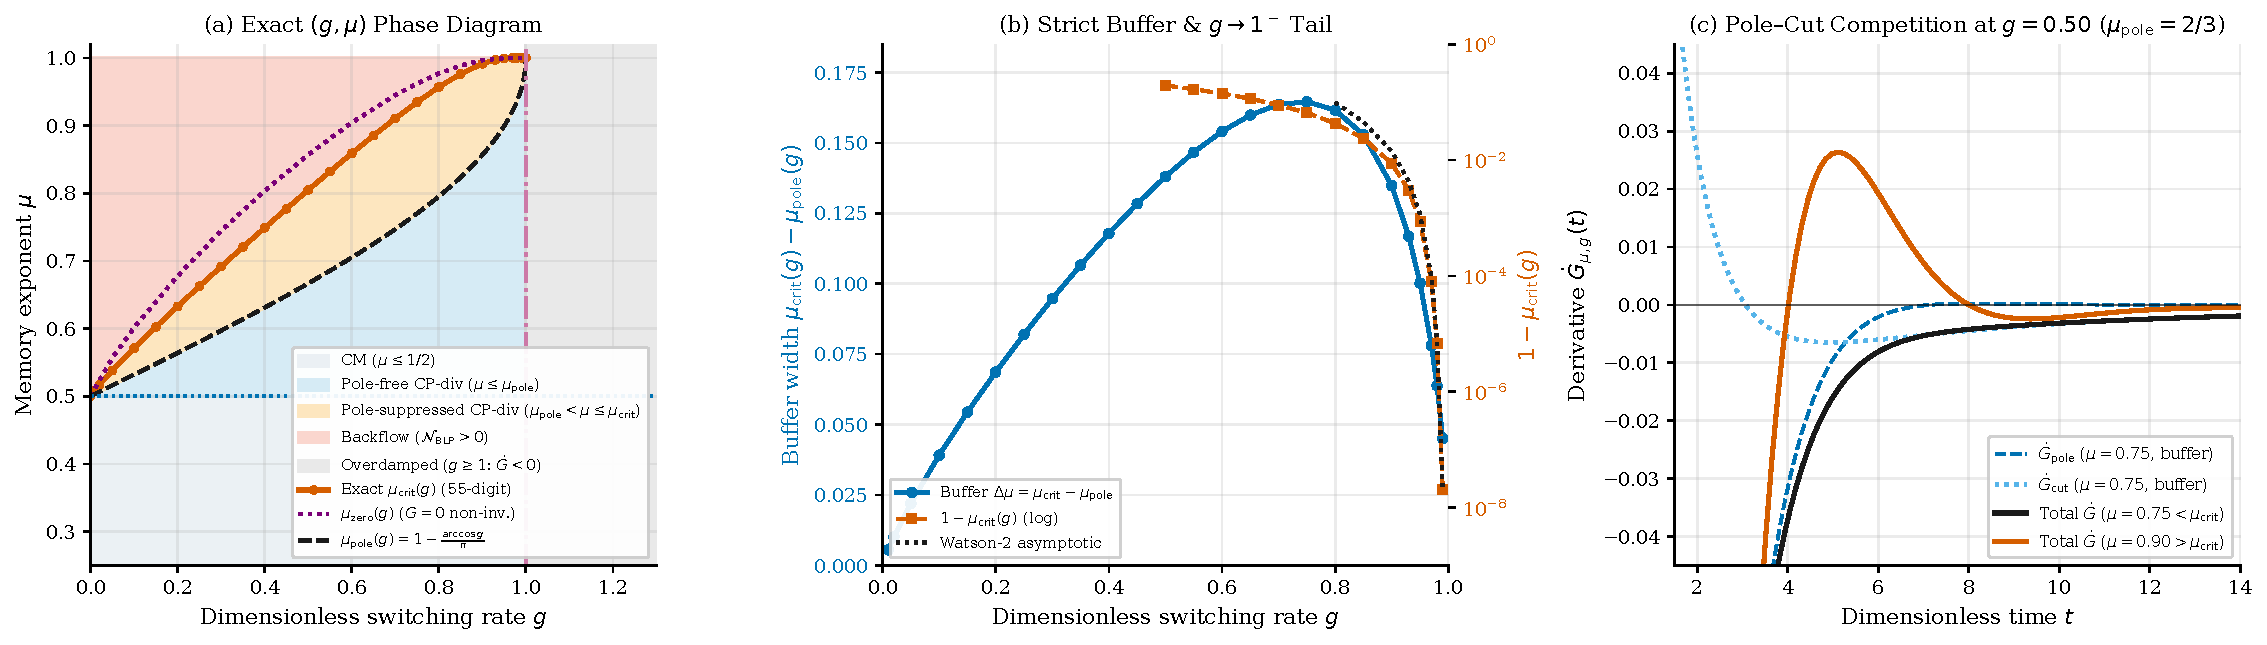
\includegraphics[width=\textwidth]{../figures/fig1_phase_diagram_unclamped.pdf}
\caption{(a) Exact $(g,\mu)$ phase diagram partitioning completely monotonic ($\mu \le 1/2$), pole-free CP-divisible ($1/2 < \mu \le \mupole(g)$), pole-suppressed CP-divisible buffer ($\mupole(g) < \mu \le \mucrit(g)$), backflow ($\NBLP > 0$), zero-crossing non-invertible ($\mu > \muzero(g)$), and overdamped ($g \ge 1$) regimes. (b) Strict buffer width $\mucrit(g)-\mupole(g)$ (left axis) and log-scale super-exponential tail $1-\mucrit(g)$ vs.\ Eq.~\eqref{eq:asymp_law} (right axis). (c) Pole-vs-cut competition $\dot{G}_{\mu,g} = \dot{G}_{\mathrm{pole}} + \dot{G}_{\mathrm{cut}}$ at $g=0.50$, comparing the buffer ($\mu=0.75$) and backflow ($\mu=0.90$) regimes.}
\label{fig:phase_diagram}
\end{figure*}

\begin{figure*}[t]
\centering
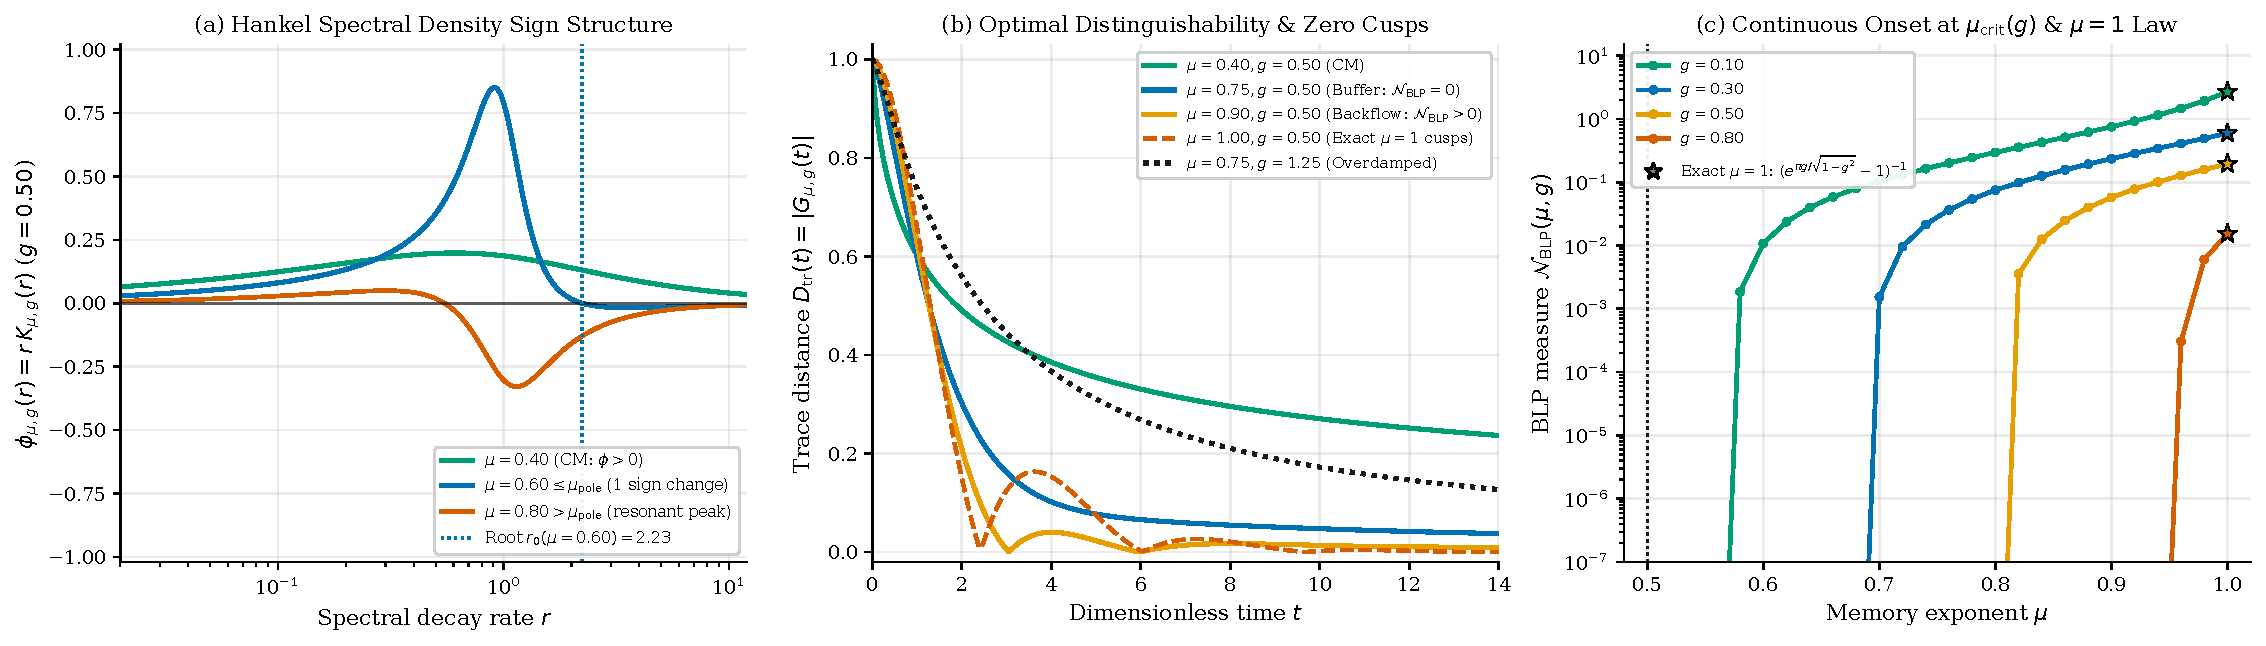
\includegraphics[width=\textwidth]{../figures/fig2_spectral_and_blp_exact.pdf}
\caption{(a) Signed spectral weight $\phi_{\mu,g}(r) = r K_{\mu,g}(r)$ at $g=0.50$ across $\mu=0.40$ (positive everywhere, CM), $\mu=0.60$ (single sign change at $r_0$), and $\mu=0.80$ (resonant cut distortion above $\mupole=2/3$). (b) Optimal trace distance $D_{\mathrm{tr}}(t) = |G_{\mu,g}(t)|$ illustrating strict decay in CM/buffer/overdamped regimes and zero-crossing cusps for $\mu > \muzero$. (c) Continuous onset of $\NBLP(\mu,g)$ at $\mucrit(g)$ terminating at the exact $\mu=1$ closed form~\eqref{eq:mu1_nblp} (stars).}
\label{fig:spectral_blp}
\end{figure*}

%==============================================================================
\section{Pauli-Semigroup Subordination and the Strict 6-Level Hierarchy}
\label{sec:hierarchy}
%==============================================================================

Evaluating a Markovian semigroup along a non-negative operational-time distribution $p_\mu(\tau,t)$ always produces a globally CPTP family whose Bloch multipliers decay monotonically, yet it does \emph{not} universally preserve CP-divisibility~\cite{Chruscinski2015PRA,Chruscinski2016PRA,Filippov2017PRA}. Below we establish the exact CP-divisibility criterion for subordinated Pauli semigroups, prove global subadditivity of the effective decay rate via Pollard log-convexity, and pinpoint the sharp breakdown at $\mustar = 0.9260578001565031$.

\subsection{Pauli-Semigroup Subordination CP-Divisibility Criterion}

Consider a general time-homogeneous qubit Pauli GKSL generator $\mathcal{L}_{\mathrm{Pauli}}(\rho) = \sum_{j=x,y,z} \frac{\gamma_j^{(0)}}{2}(\sigma_j \rho \sigma_j - \rho)$ with non-negative parent rates $\gamma_j^{(0)} \ge 0$ and Bloch eigenvalues $-\lambda_k$, where $\lambda_x = \gamma_y^{(0)} + \gamma_z^{(0)}$, $\lambda_y = \gamma_x^{(0)} + \gamma_z^{(0)}$, $\lambda_z = \gamma_x^{(0)} + \gamma_y^{(0)}$ satisfy the triangle inequalities $|\lambda_j - \lambda_k| \le \lambda_\ell \le \lambda_j + \lambda_k$ (convention used uniformly throughout). Under inverse $\mu$-stable subordination, the Bloch multipliers become $\Lambda_k(t) = \int_0^\infty \ee^{-\lambda_k \tau} p_\mu(\tau,t)\,\dd\tau = E_\mu(-\lambda_k t^\mu) \in (0,1]$, satisfying $\dot{\Lambda}_k(t) = -\gamma(\lambda_k, t)\Lambda_k(t)$ with positive Bloch-axis decay rate
\begin{align}
\label{eq:kappa_rate}
\gamma(\lambda, t) &:= -\frac{\dd}{\dd t}\ln E_\mu(-\lambda t^\mu) = \frac{1}{t}\,\kappa_\mu(\lambda t^\mu), \nonumber\\
\kappa_\mu(x) &:= \frac{x\,E_{\mu,\mu}(-x)}{E_\mu(-x)}.
\end{align}
For $\mu \in (0,1)$, $\kappa_\mu(x) \sim x/\Gamma(\mu)$ as $x \to 0^+$ (since $E_{\mu,\mu}(0) = 1/\Gamma(\mu)$ and $E_\mu(0)=1$) and $\kappa_\mu(x) = \mu\big[1 - \frac{\Gamma(1-\mu)}{\Gamma(1-2\mu)}x^{-1} + O(x^{-2})\big] \to \mu$ as $x \to \infty$ (approaching $\mu$ from below for $\mu < 1/2$ and from above for $\mu \in (1/2, 1)$). Crucially, because $E_\mu(-x) = \int_0^\infty \ee^{-rx}\,\dd\nu_\mu(r)$ is the Laplace transform of a positive non-degenerate measure $\nu_\mu$ for every $\mu \in (0,1)$~\cite{Pollard1948BAMS}, Cauchy--Schwarz guarantees strict log-convexity $\frac{\dd^2}{\dd x^2}\ln E_\mu(-x) > 0$ on $(0,\infty)$. Since $\frac{\dd}{\dd x}E_\mu(-x) = -\frac{1}{\mu}E_{\mu,\mu}(-x)$, we obtain the exact identity
\begin{align}
\label{eq:pollard_subadd}
\frac{\kappa_\mu(x)}{x} &= -\mu\,\frac{\dd}{\dd x}\ln E_\mu(-x), \nonumber\\
\frac{\dd}{\dd x}\!\left(\frac{\kappa_\mu(x)}{x}\right) &= -\mu\,\frac{\dd^2}{\dd x^2}\ln E_\mu(-x) < 0
\end{align}
for all $x > 0$ and all $\mu \in (0,1)$. Consequently, $\kappa_\mu(x)/x$ is strictly decreasing on $(0,\infty)$, which \emph{proves analytically} that $\kappa_\mu$ is strictly subadditive globally on $(0,\infty)$: $\kappa_\mu(x+y) < \kappa_\mu(x) + \kappa_\mu(y)$ for all $x, y > 0$ and all $\mu \in (0,1)$.

By Fujiwara--Algoet diagonalization~\cite{Fujiwara1999PRA} (Lean~4 Theorem~\leanid{pauli\_choi\_fujiwara\_algoet}), a time-local Pauli master equation $\dot{\rho} = \sum_{j=x,y,z} \frac{\gamma_j(t)}{2}(\sigma_j\rho\sigma_j - \rho)$ is CP-divisible iff every canonical rate $\gamma_j(t) \ge 0$ for all $t > 0$, where
\begin{equation}
\label{eq:pauli_rates_inv}
t\,\gamma_x(t) = \frac{\kappa_\mu(\lambda_y t^\mu) + \kappa_\mu(\lambda_z t^\mu) - \kappa_\mu(\lambda_x t^\mu)}{2},
\end{equation}
and cyclic permutations for $\gamma_y(t), \gamma_z(t)$. On the other hand, because every $\Lambda_k(t) > 0$ and $\dot{\Lambda}_k(t) < 0$, every subordinated Pauli semigroup is automatically globally CPTP, \textbf{strictly P-divisible} ($\NBLP = 0$) for all $\mu \in (0,1]$ and all $\gamma^{(0)} \ge 0$~\cite{Chruscinski2014PRL,Chruscinski2015PRA}, and moreover \emph{componentwise completely monotonic} on every Bloch axis (since $x \mapsto E_\mu(-x)$ is CM by Pollard's theorem~\cite{Pollard1948BAMS} and $t \mapsto \lambda_k t^\mu$ is a Bernstein function~\cite{Schilling2012Book}).

\begin{theorem}[Pauli Subordination CP-Divisibility Criterion and Symmetric-Ray Breakdown at $\mustar$]
\label{thm:pauli_subord}\mbox{}
\begin{enumerate}[label=(\alph*),leftmargin=1.5em,itemsep=2pt]
\item \textbf{Sufficient Triangle Criterion:} If $\lambda \mapsto \gamma(\lambda,t)$ (equivalently $x \mapsto \kappa_\mu(x)$) is non-decreasing and subadditive on $[0,\infty)$, then $\gamma_j(t) \ge 0$ for every axis $j \in \{x,y,z\}$ and all non-negative parent generators $\gamma^{(0)} \ge 0$, guaranteeing CP-divisibility (proved in Lean~4 over $[0,\infty)$ as Theorem~\leanid{pauli\_subordination\_cp\_sufficient}). By Eq.~\eqref{eq:pollard_subadd}, global subadditivity holds automatically for every $\mu \in (0,1)$, so non-decreasingness of $\kappa_\mu$ alone suffices.
\item \textbf{Exact Symmetric-Ray Breakdown Threshold $\mustar$:} Along the symmetric transverse family $\gamma^{(0)} = (\frac{1}{2}(L-c), \frac{c}{2}, \frac{c}{2})$ ($L > c > 0$, giving $\lambda_x = c$ and $\lambda_y = \lambda_z = L$), given the unimodal shape of $\kappa_\mu(x)$ on $\mu \in (1/2, 1)$ (unique crossing $x_0(\mu)$ of $\mu$, single maximum at $x_{\mathrm{peak}}(\mu) > x_0(\mu)$, strictly increasing on $(0, x_{\mathrm{peak}}(\mu)]$ and decreasing to $\mu^+$ on $[x_{\mathrm{peak}}(\mu), \infty)$, verified at 75 digits), there exists $t > 0$ and $L > c$ with $\gamma_x(t) < 0$ if and only if $\sup_{x>0} \kappa_\mu(x)/\mu > 2$. Solving the simultaneous criticality equations $\kappa_\mu(x) - 2\mu = 0$ and $\partial_x\kappa_\mu(x) = 0$ via 2D Newton iteration at 75- and 95-digit working precision (agreeing to $3.0 \times 10^{-77}$ with residuals $\le 1.8 \times 10^{-96}$) determines the unique critical exponent
\begin{align}
\label{eq:mustar_exact}
\mustar &= 0.9260578001565031\dots, \nonumber\\
x_* &= 3.6356687519943545\dots
\end{align}
Thus, for every $\mu > \mustar$, inverse $\mu$-stable subordination breaks CP-divisibility on an open cone of Markovian Pauli semigroups while preserving strict P-divisibility ($\NBLP = 0$) and componentwise CM of all three Bloch multipliers for all $t \ge 0$.
\item \textbf{Explicit P-Divisible Non-CP-Divisible Subordination Witness:} At $\mu = 0.95 > \mustar$ with parent rates $\gamma^{(0)} = (48, 2, 2)$ ($\lambda = (4, 50, 50)$), all global Choi eigenvalues at $t_1 = 1.0$ exceed $0.241208$ and $\NBLP = 0$, yet $\gamma_x(1.0) = -0.107248488 < 0$ ($\gamma_y(1.0)=\gamma_z(1.0)=1.094957$) and the finite-step propagator $\Phi_{1.1, 1.0}$ ($r_x = 0.812505, r_y = r_z = 0.910311$) has strictly negative Bell Choi eigenvalue $p_x = -0.002029351 < 0$ (formalized in Lean~4 Theorem~\leanid{pauli\_subord\_mu095\_counterexample}).
\end{enumerate}
\end{theorem}
\begin{proof}
For part~(a), monotonicity and subadditivity on $[0,\infty)$ imply $\lambda_x \le \lambda_y + \lambda_z \implies \kappa_\mu(\lambda_x t^\mu) \le \kappa_\mu((\lambda_y + \lambda_z)t^\mu) \le \kappa_\mu(\lambda_y t^\mu) + \kappa_\mu(\lambda_z t^\mu)$, so $t\gamma_x(t) \ge 0$ (and cyclically for $\gamma_y, \gamma_z$). For part~(b), along $\lambda_x = c$ and $\lambda_y = \lambda_z = L$, if $\sup_{x>0}\kappa_\mu(x) > 2\mu$ then choosing $x_{\mathrm{peak}}$ with $\kappa_\mu(x_{\mathrm{peak}}) > 2\mu$, setting $t = (x_{\mathrm{peak}}/c)^{1/\mu}$, and taking $L \to \infty$ sends $\kappa_\mu(Lt^\mu) \to \mu$, yielding $t\gamma_x(t) \to \mu - \frac{1}{2}\kappa_\mu(x_{\mathrm{peak}}) < 0$. Conversely, suppose $\sup_{x>0}\kappa_\mu(x) \le 2\mu$. If $L t^\mu \ge x_0(\mu)$, unimodality implies $\kappa_\mu(Lt^\mu) \ge \mu$, so $2\kappa_\mu(Lt^\mu) - \kappa_\mu(ct^\mu) \ge 2\mu - \sup_x \kappa_\mu(x) \ge 0$. In the remaining regime $0 < c t^\mu < L t^\mu < x_0(\mu) < x_{\mathrm{peak}}(\mu)$, strict monotonicity of $\kappa_\mu$ on $(0, x_{\mathrm{peak}}(\mu)]$ yields $\kappa_\mu(ct^\mu) < \kappa_\mu(Lt^\mu) < 2\kappa_\mu(Lt^\mu)$, securing $\gamma_x(t) > 0$ for all $t > 0$ and all $L > c > 0$. Part~(c) follows by direct 50-digit evaluation of Eq.~\eqref{eq:pauli_rates_inv} and $p_x = (1 + r_x - 2r_y)/4$.
\end{proof}

\begin{proposition}[Arbitrary Asymmetric Parent Triples Below $\mustar$: Exhaustive Reduction and Verification]
\label{prop:pauli_asymmetric}
Consider any triangle-valid triple $0 \le u = \lambda_y t^\mu \le v = \lambda_z t^\mu$, $w = \lambda_x t^\mu \in [v-u, v+u]$ at $\mu \in (1/2, \mustar]$ (under the unimodal profile of $\kappa_\mu$ on $(1/2, \mustar]$ with unique peak $x_{\mathrm{peak}}(\mu)$ and crossing $x_0(\mu) < x_{\mathrm{peak}}(\mu)$):
\begin{enumerate}[label=(\alph*),leftmargin=1.5em,itemsep=1pt]
\item \textbf{Large-pair regime ($u, v \ge x_0(\mu)$):} $\kappa_\mu(u) + \kappa_\mu(v) - \kappa_\mu(w) \ge 2\mu - \max_{x>0}\kappa_\mu(x) \ge 0$ holds \emph{analytically} for all $\mu \le \mustar$.
\item \textbf{Upper-branch and pre-peak regimes ($u < x_0(\mu)$ with either $w \ge v$ or $v \le x_{\mathrm{peak}}(\mu)$):} If $w \ge v$, write $w = v + \delta$ with $0 \le \delta \le u < x_0(\mu) < x_{\mathrm{peak}}(\mu)$; then analytic global subadditivity~\eqref{eq:pollard_subadd} plus monotonicity on $[0, x_{\mathrm{peak}}(\mu)]$ immediately yields $\kappa_\mu(w) \le \kappa_\mu(v) + \kappa_\mu(\delta) \le \kappa_\mu(v) + \kappa_\mu(u)$ (and if $v \ge x_{\mathrm{peak}}(\mu)$, decreasingness on $[x_{\mathrm{peak}}(\mu),\infty)$ gives $\kappa_\mu(w) \le \kappa_\mu(v)$ directly). Likewise, if $v \le x_{\mathrm{peak}}(\mu)$ and $w < v$, monotonicity on $[0, x_{\mathrm{peak}}(\mu)]$ gives $\kappa_\mu(w) \le \kappa_\mu(v) < \kappa_\mu(v) + \kappa_\mu(u)$.
\item \textbf{Remaining post-peak descent regime ($u < x_0(\mu)$, $v > x_{\mathrm{peak}}(\mu)$, $v - u \le w < v$):} By Eq.~\eqref{eq:pollard_subadd}, $\kappa_\mu(r)/r$ is strictly decreasing on $(0,\infty)$, so $\kappa_\mu(u) \ge (\mu/x_0(\mu))u$ analytically on $(0, x_0(\mu)]$. Setting $\tilde{w} := \max(w, x_{\mathrm{peak}}(\mu))$ gives $\kappa_\mu(w) - \kappa_\mu(v) \le \kappa_\mu(\tilde{w}) - \kappa_\mu(v) \le L_{\mathrm{down}}(\mu)\,u$, where $L_{\mathrm{down}}(\mu) := \sup_{x > x_{\mathrm{peak}}(\mu)} |\kappa'_\mu(x)|$. High-precision evaluation confirms $L_{\mathrm{down}}(\mu) < \mu/x_0(\mu)$ across all tested $\mu \in \{0.60, 0.70, 0.80, 0.85, 0.90, \mustar\}$, progressing monotonically from $L_{\mathrm{down}}(0.60) = 0.000876 < 0.187368 = 0.60/x_0(0.60)$ ($214\times$ margin) to $L_{\mathrm{down}}(\mustar) = 0.164221 < 0.855824 = \mustar/x_0(\mustar)$ ($5.2\times$ margin, with $x_0(\mustar) = 1.082065$ and $x_{\mathrm{inf}} = 5.413586$). Exhaustive numerical scans over $7{,}980$ 3D parent-rate configurations and $301$ triangle-boundary triples at each $\mu \in \{0.60, 0.80, 0.90, 0.925\}$ confirm zero CP-divisibility violations below $\mustar$ (Fig.~\ref{fig:pauli_ce}), whereas $\mu = 0.95$ exhibits immediate violations.
\end{enumerate}
\end{proposition}

\begin{figure*}[t]
\centering
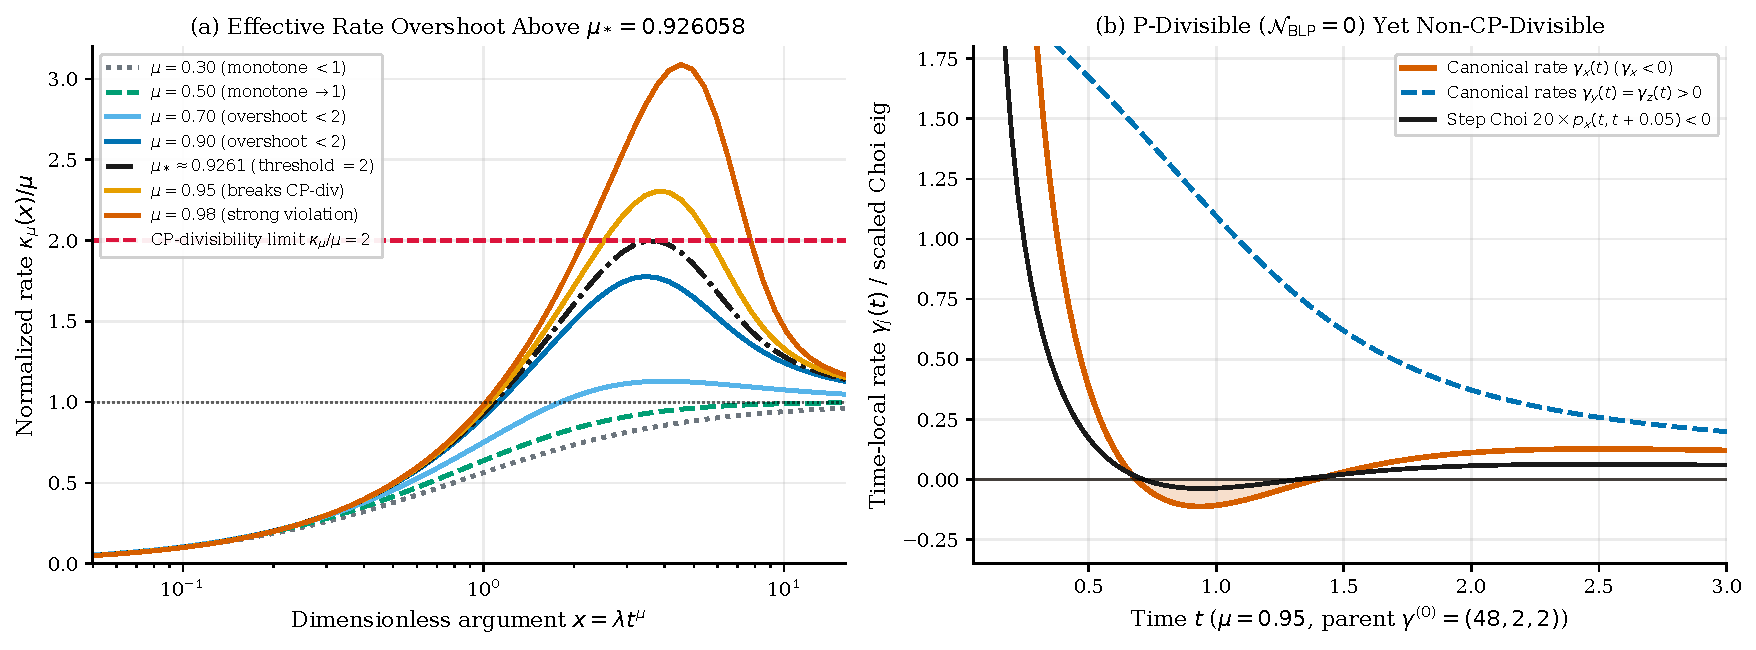
\includegraphics[width=0.95\textwidth]{../figures/fig3_pauli_subordination_counterexample.pdf}
\caption{(a) Normalized effective Pauli rate $\kappa_\mu(x)/\mu$ as a function of $x=\lambda t^\mu$: strictly monotone below $\mu=1/2$, non-monotone overshoot strictly below $2$ for $\mu \in (1/2, \mustar)$, and breaching the CP-divisibility ceiling $\kappa_\mu/\mu = 2$ above $\mustar = 0.926058$. (b) Canonical rates $\gamma_x(t) < 0$ vs.\ $\gamma_y(t)=\gamma_z(t) > 0$ and scaled negative step Choi eigenvalue $20\,p_x(t,t+0.05) < 0$ for the subordinated Pauli counterexample at $\mu=0.95$, $\gamma^{(0)} = (48,2,2)$; panel~(b) displays the finite step $\Delta t = 0.05$, whereas Theorem~\ref{thm:pauli_subord}(c) and Lean~4 certify the $\Delta t = 0.10$ interval $[1.0, 1.1]$ ($p_x = -0.00202935$).}
\label{fig:pauli_ce}
\end{figure*}

\subsection{Strict 6-Level Hierarchy of Open Quantum Dynamics}

Theorems~\ref{thm:pole_free_wedge} and~\ref{thm:pauli_subord} organize naturally into a rigorous six-level nested inclusion hierarchy for time-dependent CPTP qubit channels sharing at least one fixed state $\rho_*$:
\begin{equation}
\label{eq:hierarchy}
\mathrm{SG} \subsetneq \mathrm{CM}_{\mathrm{deph}} \subsetneq \mathrm{CP\text{-}Div} \subsetneq \mathrm{P\text{-}Div} \subsetneq \mathrm{Spohn} \subsetneq \mathrm{CPTP}.
\end{equation}
Each tier is defined strictly as follows:
\begin{itemize}[leftmargin=1.4em,itemsep=1pt]
\item $\mathrm{SG}$: time-homogeneous Markovian GKSL semigroups $\Phi_t = \ee^{t\mathcal{L}}$ (with $\Phi_t(\rho_*) = \rho_*$).
\item $\mathrm{CM}_{\mathrm{deph}}$: single-axis pure-dephasing (or isotropic depolarizing) channels whose scalar coherence factor $G(t) \in (0,1]$ is completely monotonic on $(0,\infty)$. Because $(-1)^1 \dot{G}(t) \ge 0$, the canonical rate $\gamma(t) = -\dot{G}(t)/G(t) \ge 0$ guarantees $\mathrm{CM}_{\mathrm{deph}} \subsetneq \mathrm{CP\text{-}Div}$. \emph{Crucial multi-axis caveat:} for general multi-axis Pauli channels, componentwise complete monotonicity of all three Bloch multipliers $\Lambda_k(t)$ does \emph{not} imply CP-divisibility, as refuted directly by our own Level~4a (Eternal Pauli, $\Lambda_x=\Lambda_y=\frac{1}{2}(1+\ee^{-2t}), \Lambda_z=\ee^{-2t}$) and Level~4b (Subordinated Pauli at $\mu=0.95$, $\Lambda_k(t) = E_{0.95}(-\lambda_k t^{0.95})$) witnesses below.
\item $\mathrm{CP\text{-}Div}$: CP-divisible dynamics (every intermediate propagator $\Lambda_{t,s} = \Phi_t \circ \Phi_s^{-1}$, $t \ge s \ge 0$, is CPTP).
\item $\mathrm{P\text{-}Div}$: strictly P-divisible dynamics (every $\Lambda_{t,s}$ is a positive trace-preserving map; for invertible maps, equivalent to monotonicity of all biased Helstrom operators $p\rho_1 - (1-p)\rho_2$~\cite{Wissmann2015PRA,Bae2016PRL}). On unital qubit channels (such as Levels~1--4b and~6), $\mathrm{P\text{-}Div}$ coincides with unbiased trace-distance contractivity ($\NBLP = 0$)~\cite{Chruscinski2014PRL}, whereas on non-unital maps $\mathrm{P\text{-}Div}$ is strictly stronger than $\{\NBLP = 0\}$.
\item $\mathrm{Spohn}$: global monotonicity $\frac{\dd}{\dd t} D(\Phi_t(\rho)\parallel\rho_*) \le 0$ of the Umegaki quantum relative entropy against an invariant state $\rho_*$ for every initial $\rho$~\cite{Spohn1978JMP}. Crucially, the inclusion $\mathrm{P\text{-}Div} \subseteq \mathrm{Spohn}$ holds rigorously for all positive trace-preserving intermediate propagators fixing $\rho_*$ by the M\"uller-Hermes--Reeb data-processing inequality~\cite{MullerHermes2017AHP}. Because unbiased $\NBLP = 0$ is weaker than $\mathrm{P\text{-}Div}$ for non-unital maps, any non-unital witness violating $\NBLP = 0$ \emph{a fortiori} violates $\mathrm{P\text{-}Div}$.
\end{itemize}
Enforcing relative-entropy contraction solely against one invariant state $\rho_*$ thus imposes a strictly weaker constraint than universal P-divisibility, placing $\mathrm{Spohn}$ strictly \emph{between} $\mathrm{P\text{-}Div}$ and $\mathrm{CPTP}$.

We construct an explicit continuous, piecewise-smooth ($C^0$ on $[0,\infty)$, $C^\infty$ on $[0,1)\cup(1,\infty)$ with strictly negative one-sided derivatives at the $t=1$ corner; any sufficiently sharp $C^\infty$ mollification preserves every strict inequality below) \textbf{Level~5} witness ($\mathrm{Spohn} \setminus \mathrm{P\text{-}Div}$): consider a non-unital affine Bloch flow~\cite{Ruskai2002LAA} fixing $\mathbf{r}_* = (0, 0, \frac{4}{5})^\top$ ($\rho_* = \frac{1}{2}(I + 0.8\sigma_z)$) via an initial isotropic contraction $T(t) = (1 - \frac{19}{20}t)I_3$ on $t \in [0,1]$ ($T(1) = \frac{1}{20}I_3$), followed on $t \ge 1$ by the tilted autonomous generator $\dot{\mathbf{r}} = K(\mathbf{r} - \mathbf{r}_*)$, $T(t) = \frac{1}{20}\ee^{(t-1)K}$, $\mathbf{c}(t) = (I_3 - T(t))\mathbf{r}_*$, with
\begin{equation}
\label{eq:level5_K}
K = \begin{pmatrix} -\ln 2 & 0 & \tfrac{9}{5} \\ 0 & -\ln 2 & 0 \\ 0 & 0 & -\ln\tfrac{5}{2} \end{pmatrix}.
\end{equation}
\textbf{Analytic global CPTP for all $t \ge 0$:} On $t \in [0,1]$, $\Phi_t(\rho_0) = (1-\frac{19}{20}t)\rho_0 + \frac{19}{20}t\,\rho_*$ is a convex mixture of CPTP maps ($\min_{t \ge 10^{-3}} \lambda_{\min}(J(\Phi_t)) = 4.750\times 10^{-5}$). On $t \ge 1$ ($\tau = t - 1 \ge 0$), the non-zero entries of $T(t)$ are $a(\tau) = \frac{1}{20}2^{-\tau} \in (0, \frac{1}{20}]$, $c(\tau) = \frac{1}{20}(\frac{5}{2})^{-\tau} \in (0, \frac{1}{20}]$, and $b(\tau) = \frac{1}{20}\frac{9/5}{\ln(5/4)}(2^{-\tau} - (\frac{5}{2})^{-\tau}) \in [0, 0.041277] \subset [0, \frac{1}{20}]$, with exact fixed-point shift $m_x = -\frac{4}{5}b$, $m_z = \frac{4}{5}(1-c)$. Because $(a, b, c) \in [0, \frac{1}{20}]^3$ for all $\tau \ge 0$, every row of the real symmetric $4\times 4$ Choi matrix $J(\Phi_t)$ is strictly diagonally dominant, certifying $J(\Phi_t) \ge 0$ analytically for \emph{all} $t \ge 1$ simultaneously (with $\min_{t\ge 1}\lambda_{\min}(J(\Phi_t)) = 0.04750$, and formally machine-checked across the entire box $(a,b,c) \in [0,\frac{1}{20}]^3$ in Lean~4 Theorem~\leanid{sep\_pdiv\_spohn\_uniform\_cptp}).

\textbf{P-divisibility violation and global Spohn monotonicity:} Because $\lambda_{\max}(K + K^\top) = +0.204341 > 0$, maximizing trace-distance backflow over all antipodal pure-state pairs on the Bloch sphere gives the true global maximum $\NBLP = 1.9329 \times 10^{-3} > 0$ (attained at polar angle $\theta \approx 0.6075\,\mathrm{rad}$; the interior symmetric pair $\mathbf{r}_{1,2}(0) = \mathbf{r}_* \pm 0.1\,\mathbf{u}_{\max}$ along the top eigenvector of $K + K^\top$ already yields $\NBLP^{\mathrm{pair}} = 1.1355\times 10^{-4} > 0$, plotted in Fig.~\ref{fig:hierarchy}(b)), breaking unbiased trace-distance contractivity and \emph{a fortiori} breaking $\mathrm{P\text{-}Div}$. On $t \in [0,1]$, joint convexity of relative entropy together with Klein's inequality $D((1-\alpha)\rho_0 + \alpha\rho_* \parallel \rho_*) \ge 0$ (vanishing at $\alpha=1$) enforces convex--linear monotonicity $\frac{\dd}{\dd t}D(\Phi_t(\rho_0)\parallel\rho_*) \le 0$ for all $\rho_0 \in B_1$. On $t \ge 1$, although $\dot{\mathbf{r}} = K(\mathbf{r}-\mathbf{r}_*)$ is \emph{not} Spohn-monotone on uncontracted outer-ball states ($\frac{\dd D}{\dd t} = +1.4376 > 0$ at $|\mathbf{r}|=0.99$), every initial state $\rho_0 \in B_1$ satisfies $\|\mathbf{r}_0 - \mathbf{r}_*\|_2 \le 1 + \|\mathbf{r}_*\|_2 = 1.8$ (attained at the south pole $\mathbf{r}_0 = (0,0,-1)^\top$, where $\|\mathbf{r}(1)-\mathbf{r}_*\|_2 = 0.090$). Hence the pre-contraction $T(1) = \frac{1}{20}I_3$ confines every evolved trajectory $\mathbf{r}(t) = \Phi_t(\mathbf{r}_0)$ ($t \ge 1$) strictly inside the forward-invariant contracted ball
\begin{align}
\label{eq:level5_ball}
\|\mathbf{r}(t) - \mathbf{r}_*\|_2
&\le \frac{1}{20}\big(1 + \|\mathbf{r}_*\|_2\big)\sup_{\tau\ge 0}\|\ee^{\tau K}\|_2 \nonumber\\
&= 0.093479 < 0.095
\end{align}
(exact maximum reachable distance $0.089991 \le 0.090$, Bloch norm $\|\mathbf{r}(t)\|_2 \in [0.7100, 0.8100]$). In the Bogoliubov--Kubo--Mori (BKM) Fisher metric of $\rho_*$ ($g_{xx} = \frac{5}{4}\ln 3 \approx 1.37327$, $g_{zz} = \frac{25}{9}$, Hessian--flow matrix eigenvalues $\{-6.43805, -1.90375, -0.55620\}$), Lean~4 (\leanid{sep\_pdiv\_spohn\_bkm\_vs\_blp}) interval-certifies strict negative definiteness of the linearized BKM quadratic form at $\mathbf{r}_*$, while direct nonlinear optimization of $\frac{\dd}{\dd t} D(\rho(t)\parallel\rho_*) = (\mathbf{r}(t)-\mathbf{r}_*)^\top K^\top \big(\frac{\operatorname{artanh}|\mathbf{r}|}{|\mathbf{r}|}\mathbf{r} - \frac{\operatorname{artanh} z_*}{z_*}\mathbf{r}_*\big)$ across the entire enclosing ball $\|\mathbf{r} - \mathbf{r}_*\|_2 \le 0.095$ confirms strict negativity everywhere: $\max_{|\mathbf{r}_0|=1} \frac{\dd D}{\dd t}(1^+) = -7.2260 \times 10^{-5} < 0$ on the initial Bloch sphere at $t=1^+$, $\max_{\|\mathbf{r}-\mathbf{r}_*\|_2 = 0.095}\frac{\dd D}{\dd t} = -1.9597 \times 10^{-3} < 0$ on the enclosing boundary sphere, and $\sup_{0<\|\mathbf{r}-\mathbf{r}_*\|\le 0.095}\|\mathbf{r}-\mathbf{r}_*\|_2^{-2}\frac{\dd D}{\dd t} = -0.21714 < 0$ uniformly across all non-zero shells. Thus $\Phi_t$ satisfies global Spohn monotonicity $\frac{\dd}{\dd t}D(\Phi_t(\rho_0)\parallel\rho_*) \le 0$ for every initial $\rho_0 \in B_1$ and every $t \ge 0$, while breaking $\mathrm{P\text{-}Div}$.

Table~\ref{tab:hierarchy} and Fig.~\ref{fig:hierarchy} summarize explicit quantitative witnesses---seven analytic/numerical witnesses (including both the Hall--Cresser--Li--Andersson eternal non-Markovian Pauli flow~\cite{Hall2014PRA,Megier2017SciRep} and our subordinated Pauli channel) plus machine-checked Lean~4 witnesses---strictly separating every level in~\eqref{eq:hierarchy}.

\begin{table*}[t]
\centering
\caption{Quantitative separation of all six levels of the hierarchy~\eqref{eq:hierarchy}. $\Phi_t$ is globally CPTP across every level: the rightmost column reports $\min_{t \ge 10^{-3}}\frac{1-|G(t)|}{2}$ for pure-dephasing evolutions (exact $4\times 4$ Choi spectrum $\{(1\pm G)/2, 0, 0\}$) and $\min_{t \ge 10^{-3}} \lambda_{\min}(J(\Phi_t))$ for Pauli and affine evolutions. Pure-dephasing rate and entropy-production extrema in Rows~2--3 are evaluated on the finite sampling window $t \in [10^{-3}, 40]$ for initial state $|+\rangle$.}
\label{tab:hierarchy}
\setlength{\tabcolsep}{4pt}
\resizebox{\textwidth}{!}{%
\begin{tabular}{@{}lccccccc@{}}
\toprule
Witness & Strict Level & Semigroup Defect & $\min K$ or $(-1)^2 G''$ & $\min \gamma_k(t)$ & $\NBLP$ & $\max \frac{\dd D}{\dd t}$ & $\min_{t\ge 10^{-3}} J(\Phi_t)$ \\
\midrule
1. Markov $G(t)=\ee^{-t}$ & $\mathrm{SG}$ & $0$ & $\ee^{-t} > 0$ & $+1.0000$ & $0$ & $\le 0$ & $5.00\times 10^{-4}$ \\
2. $G_{0.40, 0.20}(t)$ & $\mathrm{CM}_{\mathrm{deph}} \setminus \mathrm{SG}$ & $0.116958$ & $\min K = +7.68\times 10^{-7}$ & $+0.011888^{\sharp}$ & $0$ & $-6.33\times 10^{-5\,\sharp}$ & $2.09\times 10^{-3}$ \\
3. $G_{0.75, 0.50}(t)$ & $\mathrm{CP\text{-}Div} \setminus \mathrm{CM}_{\mathrm{deph}}$ & $0.062963$ & $(-1)^2G''(0.25) = -0.39395$ & $+0.018611^{\sharp}$ & $0$ & $-5.56\times 10^{-6\,\sharp}$ & $1.19\times 10^{-5}$ \\
4a. Eternal Pauli~\cite{Hall2014PRA}$^{*}$ & $\mathrm{P\text{-}Div} \setminus \mathrm{CP\text{-}Div}$ & n/a & comp.\ CM$^{*}$ & $-1.000000$ & $0$ & $\le 0$ & $0$ (exact) \\
4b. Subord.\ Pauli ($\mu=0.95$)$^{*}$ & $\mathrm{P\text{-}Div} \setminus \mathrm{CP\text{-}Div}$ & n/a & comp.\ CM$^{*}$ & $-0.107248$ & $0$ & $\le 0$ & $1.44\times 10^{-3\,\diamond}$ \\
5. Affine Tilt ($r_*=(0,0,0.8)$) & $\mathrm{Spohn} \setminus \mathrm{P\text{-}Div}$ & n/a & --- & $-0.204341^{\dagger}$ & $1.93\times 10^{-3\,\parallel}$ & $-7.23\times 10^{-5\,\S}$ & $4.75\times 10^{-5\,\ddagger}$ \\
6. $G_{0.90, 0.50}(t)$ & $\mathrm{CPTP} \setminus \mathrm{Spohn}$ & $0.184889$ & $\min K = -0.108941$ & $-\infty^{\flat}$ & $0.057507$ & $+0.001363$ & $1.19\times 10^{-6}$ \\
\bottomrule
\multicolumn{8}{@{}l@{}}{\scriptsize $^{*}$Multi-axis Pauli witnesses whose Bloch multipliers are componentwise CM yet lie outside $\mathrm{CM}_{\mathrm{deph}}$ and $\mathrm{CP\text{-}Div}$. $^{\diamond}$Global Choi min on $t\ge 10^{-3}$ ($0.241208$ at $t=1.0$).} \\
\multicolumn{8}{@{}l@{}}{\scriptsize $^{\sharp}$Finite-horizon $t\in[10^{-3},40]$ for $|+\rangle$ (as $t\to\infty$, $\gamma_z\sim\mu/t\to 0^+$ and $\dot{D}\to 0^-$). $^{\dagger}$Reports $-\lambda_{\max}(K+K^\top)$. $^{\parallel}$Global antipodal max (interior pair $1.14\times 10^{-4}$).} \\
\multicolumn{8}{@{}l@{}}{\scriptsize $^{\ddagger}$Uniformly $\ge 0.0475$ for all $t\ge 1$. $^{\S}$Max over $|\mathbf{r}_0|=1$ at $t=1^+$ (boundary sphere $\|\mathbf{r}-\mathbf{r}_*\|_2=0.095$: $-1.96\times 10^{-3}$; Rayleigh sup $-0.217$ on $0<\|\mathbf{r}-\mathbf{r}_*\|\le 0.095$). $^{\flat}$Diverges at $G=0$ (grid min $-20.40$).}
\end{tabular}%
}
\end{table*}

\begin{figure*}[t]
\centering
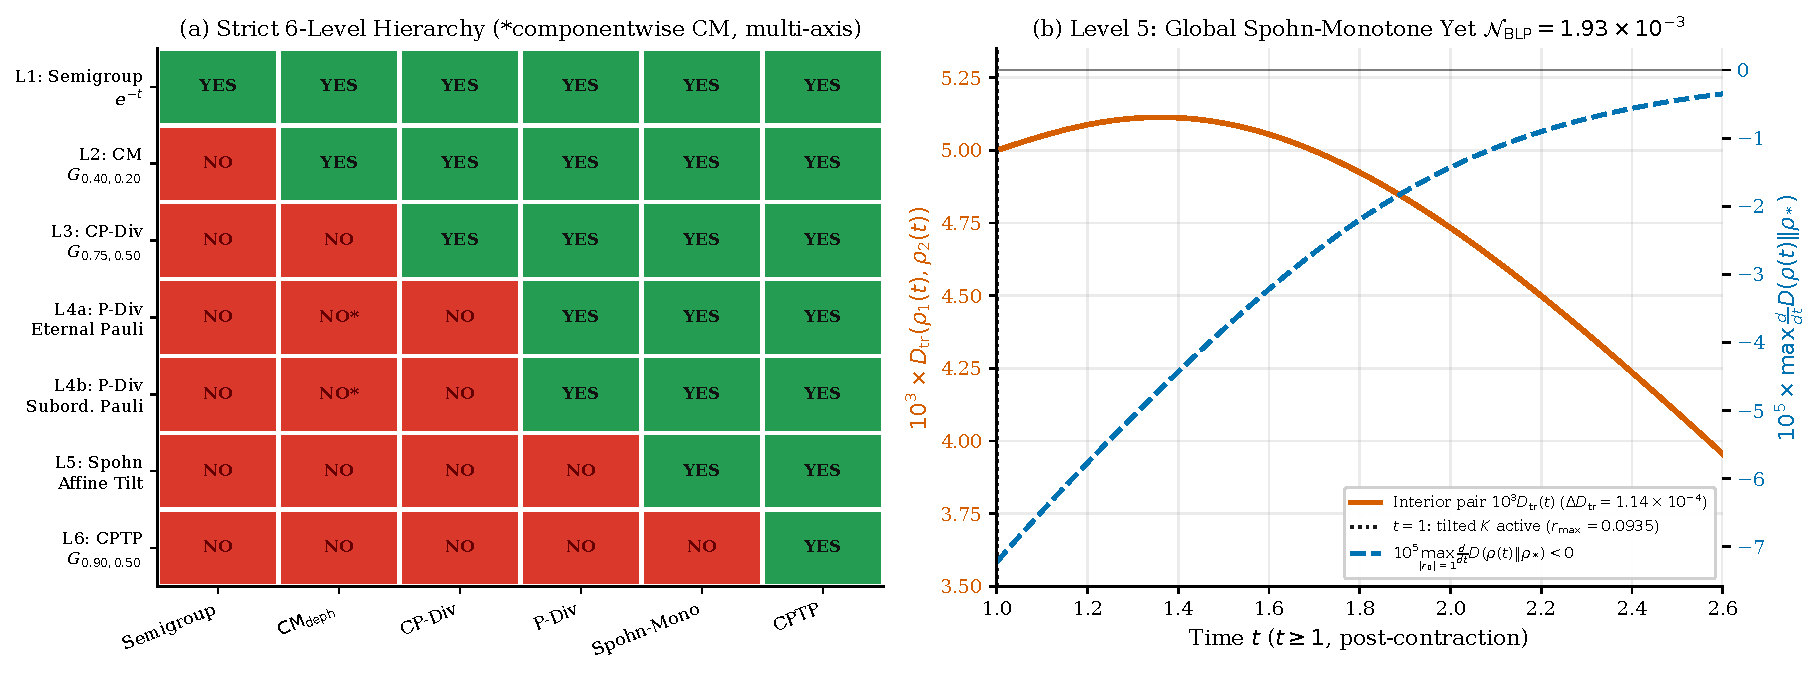
\includegraphics[width=0.95\textwidth]{../figures/fig4_hierarchy_6levels.pdf}
\caption{(a) Structural inclusion matrix confirming strict separation across all six hierarchy levels via explicit witnesses from Table~\ref{tab:hierarchy}; asterisks mark multi-axis Pauli witnesses whose Bloch multipliers are componentwise completely monotonic yet fail CP-divisibility. (b) Level~5 witness ($r_*=(0,0,0.8)$, $s=0.05$, $K_{xz}=1.8$) over the post-contraction window $t \in [1.0, 2.6]$: the interior symmetric pair $\mathbf{r}_{1,2}(0)=\mathbf{r}_*\pm 0.1\mathbf{u}_{\max}$ exhibits strict BLP trace-distance revival ($10^3 D_{\mathrm{tr}}(t)$, solid red, left axis; global antipodal maximum $\NBLP = 1.93\times 10^{-3}$), while the worst-case relative-entropy derivative over initial pure Bloch-sphere states $|\mathbf{r}_0|=1$ (evolving inside the forward-invariant contracted ball $\|\mathbf{r}-\mathbf{r}_*\|_2 \le 0.09348 < 0.095$) stays strictly negative ($10^5 \max_{|r_0|=1} \frac{\dd D}{\dd t} < 0$, dashed blue, right axis).}
\label{fig:hierarchy}
\end{figure*}

%==============================================================================
\section{Contrast with Unitary Friedrichs--Lee Microscopic Baths (\texorpdfstring{$N = 1000$}{N = 1000})}
\label{sec:friedrichs_lee}
%==============================================================================

It is essential to distinguish inverse $\mu$-stable time subordination from microscopic unitary Hamiltonian open-system models whose spectral density exhibits a power-law singularity $J(\omega) \propto \omega^{\mu-1}$ near threshold~\cite{Friedrichs1948CPAM,Lee1954PR,Garraway1997PRA}. Consider the single-excitation Friedrichs--Lee star Hamiltonian on $\mathbb{C} \oplus \mathbb{C}^N$ discretized over $N = 1000$ non-uniform Gauss--Legendre quadrature modes (eliminating uniform-grid Poincar\'e recurrences across $t \in [0, 20]$ with exact unitarity $\| |\psi(t)\rangle \| = 1 \pm 10^{-15}$):
\begin{equation}
\label{eq:fl_ham}
H = \omega_0 |e\rangle\langle e| + \sum_{k=1}^{N} \omega_k b_k^\dagger b_k + \sum_{k=1}^{N} g_k\big(|e\rangle\langle g|b_k + \mathrm{H.c.}\big),
\end{equation}
with survival amplitude $c(t) = \langle e, \mathrm{vac}| \ee^{-\ii H t} |e, \mathrm{vac}\rangle$. The continuum limit $c(t)$ obeys the linear Volterra equation $\dot{c}(t) + \ii\omega_0 c(t) = -\int_0^t \mathcal{K}(t-\tau) c(\tau)\,\dd\tau$ with $\mathcal{K}(t) = \int \dd\omega\, J(\omega) \ee^{-\ii\omega t}$. We compare three bath spectra (Table~\ref{tab:friedrichs_lee} and Fig.~\ref{fig:fl_bath}):

\begin{enumerate}[leftmargin=1.4em,itemsep=2pt]
\item \textbf{Resonant Lorentzian Bath:} Taking $J(\omega) = \frac{2g}{\pi[(\omega-\omega_0)^2 + 4g^2]}$ at $\omega_0 = 25$ (unit weight $\int J(\omega)\,\dd\omega = 1$, half-width $\lambda = 2g$), rotating-frame memory $\mathcal{K}_{\mathrm{rot}}(t) = \ee^{-2gt}$ gives $\tilde{\mathcal{K}}_{\mathrm{rot}}(s) = (s+2g)^{-1}$, and because the Lorentzian pole lies deep inside the continuum ($\omega_0 \gg g$), the rotating-frame coherence $c_{\mathrm{rot}}(t) = \ee^{\ii\omega_0 t}c(t)$ with Laplace transform $\tilde{c}_{\mathrm{rot}}(s) = [s + (s+2g)^{-1}]^{-1} = \tilde{G}_{1,g}(s)$ reproduces the exact $\mu=1$ Jaynes--Cummings propagator $G_{1,g}(t)$ with max error $1.40 \times 10^{-5}$ ($g=0.25$) and $5.61 \times 10^{-5}$ ($g=1.25$)~\cite{Garraway1997PRA}.
\item \textbf{One-Sided Power-Law Bath:} Taking $J(\omega) = \frac{\eta}{\Gamma(\mu)}\,\omega^{\mu-1}\ee^{-\omega/\omega_c}$ on $\omega > 0$ ($\eta=0.4$, $\omega_c=8$), direct integration gives $\mathcal{K}(t) = \eta(\omega_c^{-1}+\ii t)^{-\mu} \to \eta\,\ee^{-\ii\pi\mu/2} t^{-\mu}$ as $\omega_c \to \infty$, whose broadband Laplace self-energy scales as $\tilde{\mathcal{K}}(s) \sim \eta\,\Gamma(1-\mu)\,\ee^{-\ii\pi\mu/2}\,s^{\mu-1}$. Because Eq.~\eqref{eq:fl_ham} induces a generalized amplitude-damping channel ($\rho_{ee}(t) = |c(t)|^2\rho_{ee}(0)$, $\rho_{eg}(t) = c(t)\rho_{eg}(0)$) with trace distance $D_{\mathrm{tr}}(t) = \sqrt{a^2|c(t)|^4 + |b|^2|c(t)|^2}$ ($a^2 + |b|^2 \le 1$)~\cite{Laine2010PRA}, two sharp physical contrasts emerge relative to inverse-stable subordination: (i) the continuum edge $\omega = 0$ creates a real-frequency \emph{atom--photon bound state} below threshold ($E_0 = -0.65314$, $|V_{0,0}|^2 = 0.61167$ for $\omega_0=0, \mu=0.5$) trapping $|c(t)| > 1/2$, so the excited/ground pair $|e\rangle, |g\rangle$ ($D_{\mathrm{tr}} = |c(t)|^2$, $a=1$) strictly outperforms equatorial $|\pm\rangle$ ($D_{\mathrm{tr}} = |c(t)|$, $a=0$), raising optimal amplitude-damping backflow from $\NBLP(|\pm\rangle) = 0.2757$ to $\NBLP^{\mathrm{AD}} = 0.2998$ at $(\mu,\omega_0) = (0.50,0)$ and from $0.1794$ to $0.2234$ at $(0.75,0)$; and (ii) the Volterra kernel couples via $\tilde{c}(s) = [s + \ii\omega_0 + \tilde{\mathcal{K}}(s)]^{-1}$, matching the $N=1000$ unitary trace to $7.94 \times 10^{-5}$, whereas inverse $\mu$-stable subordination $E_{0.5}(-\eta t^{0.5})$ or $G_{0.5,g}(t)$ is completely monotonic with $\NBLP = 0$.
\item \textbf{Symmetric Broadband Power-Law Bath:} Taking $J_{\mathrm{sym}}(\omega) = \frac{\eta}{\Gamma(\mu)}|\omega-\omega_0|^{\mu-1}\ee^{-|\omega-\omega_0|/\omega_c}$ around $\omega_0=25$ ($\eta=0.35$, $\omega_c=12$), we obtain $\mathcal{K}_{\mathrm{rot}}(t) = 2\eta\operatorname{Re}[(\omega_c^{-1}+\ii t)^{-\mu}] \to 2\eta\cos(\frac{\pi\mu}{2})t^{-\mu}$, so its broadband Laplace transform becomes purely real and proportional to $s^{\mu-1}$, namely $\tilde{\mathcal{K}}_{\mathrm{rot}}(s) \sim c_{\mathrm{sym}}\,s^{\mu-1}$ with $c_{\mathrm{sym}} = 2\eta\cos(\frac{\pi\mu}{2})\Gamma(1-\mu)$. Inserting this into $[s + \tilde{\mathcal{K}}_{\mathrm{rot}}(s)]^{-1}$ gives $\tilde{c}_{\mathrm{rot}}(s) = s^{1-\mu}/(s^{2-\mu} + c_{\mathrm{sym}})$, whose exact inverse is the \emph{oscillatory higher-order Mittag-Leffler function} $E_{2-\mu}(-c_{\mathrm{sym}} t^{2-\mu})$ (order $2-\mu \in (1,2)$, here $E_{1.5}$ with $c_{\mathrm{sym}} = 0.87732$ at $\mu=0.5$), not the subdiffusive subordinated $E_\mu(-c t^\mu)$ (order $\mu < 1$). The $N=1000$ unitary evolution matches the continuum Volterra solution to $1.57 \times 10^{-4}$ and displays oscillatory coherent revivals ($\NBLP^{\mathrm{AD}} = \NBLP(|\pm\rangle) = 0.3951$ on $t \in [0, 20]$), confirming that $\mu \in (0,1)$ fractional subordination requires stochastic operational-time randomization rather than a static real-frequency Ohmic or sub-Ohmic bath.
\end{enumerate}

\begin{table*}[t]
\centering
\caption{Quantitative comparison of $N=1000$ Gauss--Legendre unitary Friedrichs--Lee simulations against continuum Volterra solutions ($E_{2-\mu}$) and inverse $\mu$-stable subordination over $t \in [0, 20]$ (fine grid $\Delta t = 0.002$; unitarity conserved to $1 \pm 10^{-15}$). Both equatorial coherence backflow $\NBLP(|\pm\rangle)$ and exact amplitude-damping optimal backflow $\NBLP^{\mathrm{AD}} = \max_{a^2+|b|^2=1}\int_{\dot{D}>0}\dot{D}\,\dd t$ are reported.}
\label{tab:friedrichs_lee}
\setlength{\tabcolsep}{4pt}
\resizebox{\textwidth}{!}{%
\begin{tabular}{@{}lcccccc@{}}
\toprule
Bath Model & $(\mu, \omega_0)$ & Param & Bound $E_0 / |V_{0,0}|^2$ & $\max|\Delta_{\mathrm{FL-Volterra}}|$ & $\NBLP(|\pm\rangle) / \NBLP^{\mathrm{AD}}$ & Subordination Counterpart \\
\midrule
Lorentzian ($\omega_0=25$) & $(1.0, 25)$ & $g=0.25$ & none & $1.40 \times 10^{-5}$ (vs $G_{1,0.25}$) & $0.7929 / 0.7929^{\S}$ & Exact $\mu=1$ $G_{1,0.25}(t)$ \\
Lorentzian ($\omega_0=25$) & $(1.0, 25)$ & $g=1.25$ & none & $5.61 \times 10^{-5}$ (vs $G_{1,1.25}$) & $0 / 0$ & Exact $\mu=1$ $G_{1,1.25}(t)$ \\
One-sided $\omega^{\mu-1}\ee^{-\omega/\omega_c}/\Gamma(\mu)$ & $(0.50, 0)$ & $\eta=0.4$ & $-0.6531 / 0.6117$ & $7.94 \times 10^{-5}$ & $0.2757 / 0.2998^{*}$ & $E_{0.5}(-\eta t^{0.5})$ ($\NBLP=0$) \\
One-sided $\omega^{\mu-1}\ee^{-\omega/\omega_c}/\Gamma(\mu)$ & $(0.50, 1)$ & $\eta=0.4$ & $-0.2308 / 0.2424$ & $1.16 \times 10^{-4}$ & $0.3521 / 0.3521$ & $G_{0.5,0.3}(t)$ ($\NBLP=0$) \\
One-sided $\omega^{\mu-1}\ee^{-\omega/\omega_c}/\Gamma(\mu)$ & $(0.75, 0)$ & $\eta=0.4$ & $-0.7066 / 0.6674$ & $1.22 \times 10^{-4}$ & $0.1794 / 0.2234^{*}$ & $G_{0.75,0.50}(t)$ (Buffer $\NBLP=0$) \\
One-sided $\omega^{\mu-1}\ee^{-\omega/\omega_c}/\Gamma(\mu)$ & $(0.75, 1)$ & $\eta=0.4$ & $-0.2152 / 0.2972$ & $1.67 \times 10^{-4}$ & $0.1902 / 0.1902$ & $G_{0.75,0.50}(t)$ (Buffer $\NBLP=0$) \\
Symmetric $|\omega-\omega_0|^{\mu-1}\ee^{-\cdot}/\Gamma(\mu)$ & $(0.50, 25)$ & $c_{\mathrm{sym}}=0.8773^{\ddagger}$ & none & $1.57 \times 10^{-4}$ & $0.3951 / 0.3951$ & Broadband $E_{1.5}$ vs.\ CM $E_{0.5}$ \\
Symmetric $|\omega-\omega_0|^{\mu-1}\ee^{-\cdot}/\Gamma(\mu)$ & $(0.75, 25)$ & $c_{\mathrm{sym}}=0.9712^{\ddagger}$ & none & $4.46 \times 10^{-4}$ & $0.1306 / 0.1306$ & Broadband $E_{1.25}$ oscillations \\
\bottomrule
\multicolumn{7}{@{}l@{}}{\scriptsize $^{\S}$Measured on $t\in[0,20]$ at $\Delta t = 0.002$ (exact $t\to\infty$ closed form $\NBLP(1,0.25) = 0.7997$). $^{*}$Bound state $|c(t)|>1/2$ makes $|e\rangle,|g\rangle$ ($a=1$) optimal over $|\pm\rangle$. $^{\ddagger}$$\eta=0.35, \omega_c=12$: $c_{\mathrm{sym}}=2\eta\cos(\pi\mu/2)\Gamma(1-\mu)$.}
\end{tabular}%
}
\end{table*}

\begin{figure*}[t]
\centering
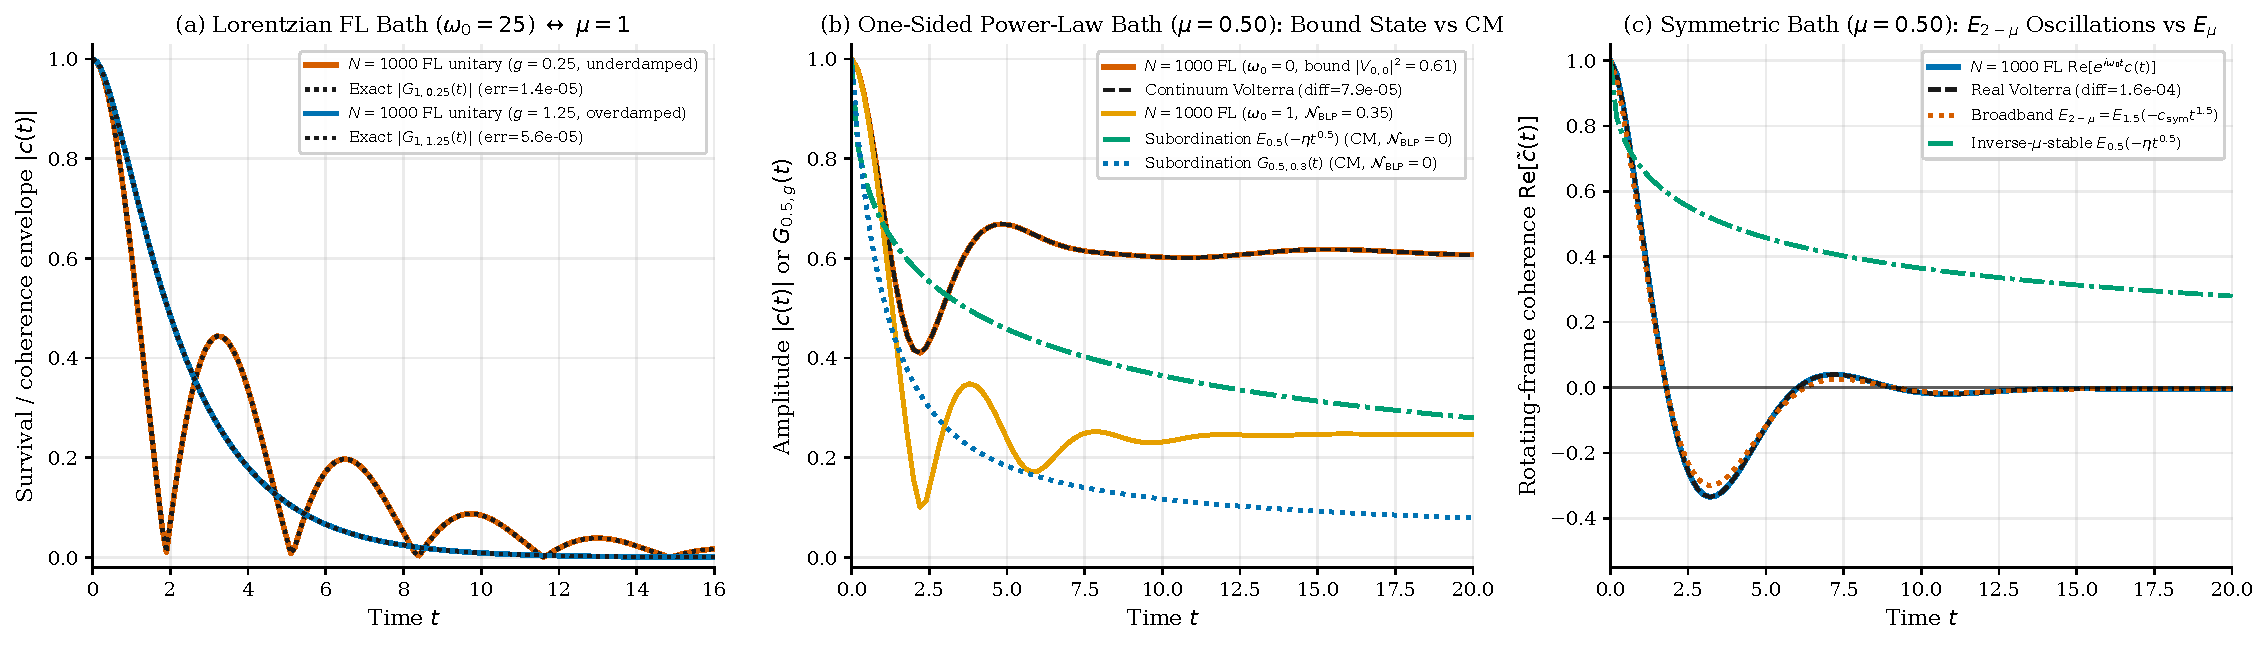
\includegraphics[width=\textwidth]{../figures/fig5_friedrichs_lee_unitary.pdf}
\caption{$N=1000$ non-uniform Gauss--Legendre unitary Friedrichs--Lee dynamics vs.\ continuum Volterra equations and subordination. (a) Resonant Lorentzian bath ($\omega_0=25$) matching $\mu=1$ $G_{1,g}(t)$ to $\le 5.6\times 10^{-5}$. (b) One-sided singular power-law bath ($\mu=0.50$) forming a bound state ($|V_{0,0}|^2=0.61$) with $\NBLP^{\mathrm{AD}} = 0.2998$ ($\NBLP(|\pm\rangle)=0.2757$), contrasted against completely monotonic $E_{0.5}$ and $G_{0.5,0.3}$ subordination. (c) Symmetric broadband power-law bath generating oscillatory $E_{2-\mu} = E_{1.5}$ coherence reversals ($\NBLP=0.3951$), distinct from $E_{0.5}$ time subordination.}
\label{fig:fl_bath}
\end{figure*}

%==============================================================================
\section{Formal Machine-Checked Verification in Pure Lean~4}
\label{sec:lean}
%==============================================================================

To eliminate sign-convention errors, hidden branch-cut ambiguities, and unverified algebraic positivity steps, we formalized the algebraic, functional-positivity, geometric-sum, and finite-dimensional $4\times 4$ Choi separation core of this work in pure Lean~4.16.0 (\leanid{Paper2\_Subordination.lean}, 2,935 lines), using zero external libraries (no Mathlib), zero \texttt{sorry}/\texttt{admit}, zero custom axioms, and no \texttt{native\_decide}/\texttt{Lean.ofReduceBool} (every rational inequality uses kernel-verified \texttt{decide} over an explicitly constructed quotient field \leanid{Q}). Continuous integrals are abstracted via an explicit \leanid{PositiveLinearFunctional} \texttt{structure} parameterized by an admissible linear subspace predicate \leanid{Adm : (D -> F) -> Prop} closed under addition and scalar multiplication, so that atomless Lebesgue or Riemann integration on $C((0,\infty)) \cap L^1((0,\infty))$ is a genuine model of Lemma~\ref{lem:ssc_positivity} without axiomatically importing measure theory.

It is important to delineate transparently the exact boundary between what is proved universally in Lean~4 versus what relies on 50--95-digit \texttt{mpmath} transcendental evaluation:
{\raggedright
\begin{itemize}[leftmargin=1.4em,itemsep=2pt]
\item \textbf{Universal algebraic and functional proofs over arbitrary ordered/commutative fields (18 headline theorems, 14 axiom-free):} Exact Hankel numerator identities (\leanid{hankel\_propagator\_numerator\_im}, \leanid{hankel\_derivative\_numerator\_im}), CM positivity and single-sign-change inequalities (\leanid{cm\_spectral\_numerator\_pos}, \leanid{single\_sign\_change\_below}, \leanid{single\_sign\_change\_above}), full overdamped and underdamped root/pole classification (\leanid{overdamped\_no\_nonneg\_real\_root}, \leanid{real\_root\_strictly\_neg}, \leanid{underdamped\_no\_real\_roots}, \leanid{underdamped\_complex\_root\_char}, \leanid{pole\_wedge\_boundary\_iff}, \leanid{subdiffusive\_always\_pole\_free}), the abstract Single-Sign-Change Positivity Theorem (\leanid{single\_sign\_change\_integral\_pos}), the $\mu=1$ geometric partial-sum and tail identities (\leanid{geom\_partial\_sum\_identity}, \leanid{geom\_tail\_archimedean\_bound}), Fujiwara--Algoet $4\times 4$ Choi diagonalization (\leanid{pauli\_choi\_fujiwara\_algoet}), the sufficient Pauli subordination criterion over $[0,\infty)$ (\leanid{pauli\_subordination\_cp\_sufficient}), strict monotonicity of the CP-divisible rational witness (\leanid{gRatCP\_strictly\_decreasing}), and the universal Gershgorin sum-of-rank-1 non-unital $4\times 4$ Choi positivity theorem (\leanid{choiNonUnital\_isPSD\_of\_gershgorin}).
\item \textbf{Rational interval and continuum-box certificates over \leanid{Q} (4 headline theorems):} The finite-step $\mu=0.95$ Pauli Choi negativity interval certificate (\leanid{pauli\_subord\_mu095\_counterexample}), exact fixed-point preservation for all $(a,b,c) \in \mathbb{Q}^3$ (\leanid{sep\_pdiv\_spohn\_fixed\_point}), the uniform global CPTP certificate across the entire box $(a,b,c) \in [0, 1/20]^3$ covering every $t \ge 1$ of the Level~5 channel simultaneously (\leanid{sep\_pdiv\_spohn\_uniform\_cptp}), and the interval-certified BKM Sylvester negative definiteness vs.\ Euclidean BLP expansion witness (\leanid{sep\_pdiv\_spohn\_bkm\_vs\_blp}).
\item \textbf{Exact single-point rational separation witnesses over \leanid{Q} (6 headline theorems):} Concrete hierarchy-separation witnesses (\leanid{sep\_semigroup\_cm}, \leanid{sep\_cm\_cpdiv\_midpoint\_nonconvex}, \leanid{sep\_cpdiv\_pdiv\_eternal}, \leanid{sep\_pdiv\_spohn\_phi1\_cptp}, \leanid{sep\_pdiv\_spohn\_phi2\_cptp} with exact fixed-point shift $m_z = 479/625 = 0.7664$ deduced from \leanid{sep\_pdiv\_spohn\_uniform\_cptp}, and \leanid{sep\_spohn\_cptp}). The transcendental evaluations ($E_\mu, \ln, \exp, \operatorname{artanh}$) anchoring the numerical intervals and the nonlinear global Spohn check across the enclosing ball $\|\mathbf{r}-\mathbf{r}_*\|_2 \le 0.095$ are established at 50--95 decimal digits in Sections~\ref{sec:phase_boundary}--\ref{sec:hierarchy}.
\end{itemize}
}
Kernel inspection via \texttt{Lean.collectAxioms} across all 150 explicitly authored public theorems (plus 46 private lemmas, totaling 196 authored theorems and 211 public kernel \texttt{thmInfo} entries including compiler-generated projections and proof obligations, of which 165 depend on zero axioms)---and all 28 headline \texttt{\#print axioms} declarations logged in \texttt{axioms\_check.txt} and summarized in Table~\ref{tab:lean_ledger}---confirms zero disallowed axioms (strictly subsets of \texttt{propext}, \texttt{Classical.choice}, \texttt{Quot.sound}), with 14 of the 28 headline theorems depending on no axioms whatsoever.

\begin{table*}[t]
\centering
\caption{Lean~4.16.0 verification ledger (\leanid{Paper2\_Subordination.lean}, 2,935 lines, pure \texttt{Init}, zero \texttt{sorry}, zero \texttt{Lean.ofReduceBool}, zero custom axioms across 150 authored public theorems / 211 public kernel \texttt{thmInfo} entries and all 28 headline \texttt{\#print axioms} checks, 14/28 axiom-free).}
\label{tab:lean_ledger}
\setlength{\tabcolsep}{4pt}
\resizebox{\textwidth}{!}{%
\begin{tabular}{@{}llll@{}}
\toprule
Mathematical Component & Formal Lean~4 Theorem(s) & Proof Scope & Axioms \\
\midrule
Hankel propagator \& $-\dot{G}$ numerator (Eq.~\eqref{eq:im_exact_step}) & \leanid{hankel\_propagator\_numerator\_im}, \leanid{hankel\_derivative\_numerator\_im} & Universal algebraic & None \\
CM positivity ($\mu \le 1/2$) \& unique crossing & \leanid{cm\_spectral\_numerator\_pos}, \leanid{single\_sign\_change\_below/above} & Universal algebraic & None \\
Root classification ($g \ge 1$ vs $g < 1$) & \leanid{overdamped\_no\_nonneg\_real\_root}, \leanid{real\_root\_strictly\_neg}, \leanid{underdamped\_no\_real\_roots}, \leanid{subdiffusive\_always\_pole\_free} & Universal algebraic & None \\
Pole entry $\mupole(g)$ iff condition & \leanid{pole\_wedge\_boundary\_iff}, \leanid{underdamped\_complex\_root\_char} & Universal algebraic & \texttt{propext} / Std \\
Single-Sign-Change Positivity (Lemma~\ref{lem:ssc_positivity}) & \leanid{single\_sign\_change\_integral\_pos} (admissible subspace \leanid{Adm}) & Universal functional & \texttt{Quot.sound} \\
Exact $\mu=1$ geometric series (Theorem~\ref{thm:asymptotic_and_mu1}(b)) & \leanid{geom\_partial\_sum\_identity}, \leanid{geom\_tail\_archimedean\_bound} & Universal algebraic & None \\
Fujiwara--Algoet $4\times 4$ Choi & \leanid{pauli\_choi\_fujiwara\_algoet} & Universal algebraic & None \\
Pauli subordination criterion (Theorem~\ref{thm:pauli_subord}(a)) & \leanid{pauli\_subordination\_cp\_sufficient} ($[0,\infty)$ domain) & Universal algebraic & None \\
Pauli $\mu=0.95$ CP-breaking witness & \leanid{pauli\_subord\_mu095\_counterexample} & Rational interval & Std \\
Monotonicity of rational CP-Div witness & \leanid{gRatCP\_strictly\_decreasing} & Universal algebraic & \texttt{propext} \\
Hierarchy: $\mathrm{SG} \subsetneq \mathrm{CM}_{\mathrm{deph}} \subsetneq \mathrm{CP\text{-}Div} \subsetneq \mathrm{P\text{-}Div}$ & \leanid{sep\_semigroup\_cm}, \leanid{sep\_cm\_cpdiv\_midpoint\_nonconvex}, \leanid{sep\_cpdiv\_pdiv\_eternal} & Single-point rational & Std \\
Level~5 Gershgorin global CPTP ($4\times 4$ PSD) & \leanid{choiNonUnital\_isPSD\_of\_gershgorin} & Universal algebraic & None \\
Level~5 fixed point, all-$t\ge 1$ box CPTP, BKM & \leanid{sep\_pdiv\_spohn\_fixed\_point}, \leanid{sep\_pdiv\_spohn\_uniform\_cptp}, \leanid{sep\_pdiv\_spohn\_bkm\_vs\_blp} & Rational box/interval & Std \\
Level~5 snapshots \& $\mathrm{Spohn} \subsetneq \mathrm{CPTP}$ & \leanid{sep\_pdiv\_spohn\_phi1\_cptp}, \leanid{sep\_pdiv\_spohn\_phi2\_cptp}, \leanid{sep\_spohn\_cptp} & Single-point rational & Std \\
\bottomrule
\end{tabular}%
}
\end{table*}

%==============================================================================
\section{Conclusion}
\label{sec:conclusion}
%==============================================================================

By anchoring inverse $\mu$-stable operational-time subordination in an exact bipartite Markovian random-telegraph semigroup and pairing contour analysis with 55-digit 2D Newton root finding and pure Lean~4 machine verification, we have established the complete phase diagram separating complete monotonicity, CP-divisibility, P-divisibility, trace-distance backflow, and global complete positivity. Rather than triggering information backflow immediately upon pole entry at $\mupole(g) = 1 - \arccos(g)/\pi$, the negative algebraic branch-cut tail stabilizes strict CP-divisibility across a finite buffer wedge $\mu \in (\mupole(g), \mucrit(g)]$ that closes super-exponentially at $g \to 1^-$ as $\frac{\pi^2}{2\ee(1-g^2)}\exp(-\pi g/\sqrt{1-g^2})$ and joins continuously onto the exact $\mu=1$ geometric-series law $\NBLP(1,g) = (\ee^{\pi g/\sqrt{1-g^2}}-1)^{-1}\mathbf{1}_{g<1}$. Moreover, operational-time subordination of Markovian Pauli semigroups preserves P-divisibility and componentwise complete monotonicity universally while breaking CP-divisibility above the 55-digit threshold $\mustar = 0.9260578001565031$, and non-unital affine flows with analytically certified global CPTP show that Spohn relative-entropy monotonicity is strictly weaker than P-divisibility, constructively separating all six structural tiers $\mathrm{SG} \subsetneq \mathrm{CM}_{\mathrm{deph}} \subsetneq \mathrm{CP\text{-}Div} \subsetneq \mathrm{P\text{-}Div} \subsetneq \mathrm{Spohn} \subsetneq \mathrm{CPTP}$ in open quantum dynamics.

\begin{acknowledgments}
The author thanks Sri Chaitanya Educational Institutions for institutional support and acknowledges open-source contributors to the Lean~4 theorem prover and Python scientific ecosystem (\texttt{mpmath}, \texttt{NumPy}, \texttt{SciPy}).
\end{acknowledgments}

\section*{Data Availability}
{\def\UrlBreaks{\do\/\do-}%
All arbitrary-precision numerical scripts (55- to 95-digit 2D Newton solvers, Pauli-subordination and six-level hierarchy verifiers, and $N=1000$ unitary Friedrichs--Lee simulations), verified strict RFC-8259 JSON/CSV datasets, vector figure scripts, and the self-contained pure Lean~4.16.0 formalization (\leanid{Paper2\_Subordination.lean}, \texttt{axioms\_check.txt}) that support the findings of this study are openly available in the Supplemental Material and at the public GitHub repository \url{https://github.com/Mehardeep-Singh-GG/subordinated-oqs-phase-boundary} (release \texttt{v1.0.0}).%
}

{\raggedright
\begin{thebibliography}{99}

\bibitem{Breuer2009PRL}
H.-P.~Breuer, E.-M.~Laine, and J.~Piilo,
Measure for the degree of non-Markovian behavior of quantum processes in open systems,
\emph{Phys.\ Rev.\ Lett.} \textbf{103}, 210401 (2009),
\href{https://doi.org/10.1103/PhysRevLett.103.210401}{doi:10.1103/PhysRevLett.103.210401}.

\bibitem{Laine2010PRA}
E.-M.~Laine, J.~Piilo, and H.-P.~Breuer,
Measure for the non-Markovianity of quantum processes,
\emph{Phys.\ Rev.\ A} \textbf{81}, 062115 (2010),
\href{https://doi.org/10.1103/PhysRevA.81.062115}{doi:10.1103/PhysRevA.81.062115}.

\bibitem{Rivas2010PRL}
\'A.~Rivas, S.~F.~Huelga, and M.~B.~Plenio,
Entanglement and non-Markovianity of quantum evolutions,
\emph{Phys.\ Rev.\ Lett.} \textbf{105}, 050403 (2010),
\href{https://doi.org/10.1103/PhysRevLett.105.050403}{doi:10.1103/PhysRevLett.105.050403}.

\bibitem{Chruscinski2011PRA}
D.~Chru\'sci\'nski, A.~Kossakowski, and \'A.~Rivas,
Measures of non-Markovianity: Divisibility versus backflow of information,
\emph{Phys.\ Rev.\ A} \textbf{83}, 052128 (2011),
\href{https://doi.org/10.1103/PhysRevA.83.052128}{doi:10.1103/PhysRevA.83.052128}.

\bibitem{Rivas2014RPP}
\'A.~Rivas, S.~F.~Huelga, and M.~B.~Plenio,
Quantum non-Markovianity: characterization, quantification and detection,
\emph{Rep.\ Prog.\ Phys.} \textbf{77}, 094001 (2014),
\href{https://doi.org/10.1088/0034-4885/77/9/094001}{doi:10.1088/0034-4885/77/9/094001}.

\bibitem{Breuer2016RMP}
H.-P.~Breuer, E.-M.~Laine, J.~Piilo, and B.~Vacchini,
Colloquium: Non-Markovian dynamics in open quantum systems,
\emph{Rev.\ Mod.\ Phys.} \textbf{88}, 021002 (2016),
\href{https://doi.org/10.1103/RevModPhys.88.021002}{doi:10.1103/RevModPhys.88.021002}.

\bibitem{Hall2014PRA}
M.~J.~W.~Hall, J.~D.~Cresser, L.~Li, and E.~Andersson,
Canonical form of master equations and characterization of non-Markovianity,
\emph{Phys.\ Rev.\ A} \textbf{89}, 042120 (2014),
\href{https://doi.org/10.1103/PhysRevA.89.042120}{doi:10.1103/PhysRevA.89.042120}.

\bibitem{Chruscinski2014PRL}
D.~Chru\'sci\'nski and S.~Maniscalco,
Degree of non-Markovianity of quantum evolution,
\emph{Phys.\ Rev.\ Lett.} \textbf{112}, 120404 (2014),
\href{https://doi.org/10.1103/PhysRevLett.112.120404}{doi:10.1103/PhysRevLett.112.120404}.

\bibitem{Wissmann2015PRA}
S.~Wi\ss mann, H.-P.~Breuer, and B.~Vacchini,
Generalized trace-distance measure connecting quantum and classical non-Markovianity,
\emph{Phys.\ Rev.\ A} \textbf{92}, 042108 (2015),
\href{https://doi.org/10.1103/PhysRevA.92.042108}{doi:10.1103/PhysRevA.92.042108}.

\bibitem{Bae2016PRL}
J.~Bae and D.~Chru\'sci\'nski,
Operational characterization of divisibility of dynamical maps,
\emph{Phys.\ Rev.\ Lett.} \textbf{117}, 050403 (2016),
\href{https://doi.org/10.1103/PhysRevLett.117.050403}{doi:10.1103/PhysRevLett.117.050403}.

\bibitem{Filippov2017PRA}
S.~N.~Filippov, J.~Piilo, S.~Maniscalco, and M.~Ziman,
Divisibility of quantum dynamical maps and collision models,
\emph{Phys.\ Rev.\ A} \textbf{96}, 032111 (2017),
\href{https://doi.org/10.1103/PhysRevA.96.032111}{doi:10.1103/PhysRevA.96.032111}.

\bibitem{Lindblad1976}
G.~Lindblad,
On the generators of quantum dynamical semigroups,
\emph{Commun.\ Math.\ Phys.} \textbf{48}, 119--130 (1976),
\href{https://doi.org/10.1007/BF01608499}{doi:10.1007/BF01608499}.

\bibitem{Gorini1976JMP}
V.~Gorini, A.~Kossakowski, and E.~C.~G.~Sudarshan,
Completely positive dynamical semigroups of $N$-level systems,
\emph{J.\ Math.\ Phys.} \textbf{17}, 821--825 (1976),
\href{https://doi.org/10.1063/1.522979}{doi:10.1063/1.522979}.

\bibitem{Spohn1978JMP}
H.~Spohn,
Entropy production for quantum dynamical semigroups,
\emph{J.\ Math.\ Phys.} \textbf{19}, 1227--1230 (1978),
\href{https://doi.org/10.1063/1.523789}{doi:10.1063/1.523789}.

\bibitem{Budini2004PRA}
A.~A.~Budini,
Stochastic representation of a class of non-Markovian completely positive evolutions,
\emph{Phys.\ Rev.\ A} \textbf{69}, 042107 (2004),
\href{https://doi.org/10.1103/PhysRevA.69.042107}{doi:10.1103/PhysRevA.69.042107}.

\bibitem{Daffer2004PRA}
S.~Daffer, K.~W\'odkiewicz, J.~D.~Cresser, and J.~K.~McIver,
Depolarizing channel as a completely positive map with memory,
\emph{Phys.\ Rev.\ A} \textbf{70}, 010304(R) (2004),
\href{https://doi.org/10.1103/PhysRevA.70.010304}{doi:10.1103/PhysRevA.70.010304}.

\bibitem{Shabani2005PRA}
A.~Shabani and D.~A.~Lidar,
Completely positive post-Markovian master equation via a measurement approach,
\emph{Phys.\ Rev.\ A} \textbf{71}, 020101(R) (2005),
\href{https://doi.org/10.1103/PhysRevA.71.020101}{doi:10.1103/PhysRevA.71.020101}.

\bibitem{Breuer2008PRL}
H.-P.~Breuer and B.~Vacchini,
Quantum semi-Markov processes,
\emph{Phys.\ Rev.\ Lett.} \textbf{101}, 140402 (2008),
\href{https://doi.org/10.1103/PhysRevLett.101.140402}{doi:10.1103/PhysRevLett.101.140402}.

\bibitem{Breuer2009PRE}
H.-P.~Breuer and B.~Vacchini,
Structure of completely positive quantum master equations with memory kernel,
\emph{Phys.\ Rev.\ E} \textbf{79}, 041147 (2009),
\href{https://doi.org/10.1103/PhysRevE.79.041147}{doi:10.1103/PhysRevE.79.041147}.

\bibitem{Vacchini2013PRA}
B.~Vacchini,
Non-Markovian master equations from piecewise dynamics,
\emph{Phys.\ Rev.\ A} \textbf{87}, 030101(R) (2013),
\href{https://doi.org/10.1103/PhysRevA.87.030101}{doi:10.1103/PhysRevA.87.030101}.

\bibitem{Addis2014PRA}
C.~Addis, B.~Bylicka, D.~Chru\'sci\'nski, and S.~Maniscalco,
Comparative study of non-Markovianity measures in exactly solvable one- and two-qubit models,
\emph{Phys.\ Rev.\ A} \textbf{90}, 052103 (2014),
\href{https://doi.org/10.1103/PhysRevA.90.052103}{doi:10.1103/PhysRevA.90.052103}.

\bibitem{Chruscinski2015PRA}
D.~Chru\'sci\'nski and F.~A.~Wudarski,
Non-Markovianity degree for random unitary evolution,
\emph{Phys.\ Rev.\ A} \textbf{91}, 012104 (2015),
\href{https://doi.org/10.1103/PhysRevA.91.012104}{doi:10.1103/PhysRevA.91.012104}.

\bibitem{Chruscinski2016PRA}
D.~Chru\'sci\'nski and A.~Kossakowski,
Sufficient conditions for a memory-kernel master equation,
\emph{Phys.\ Rev.\ A} \textbf{94}, 020103(R) (2016),
\href{https://doi.org/10.1103/PhysRevA.94.020103}{doi:10.1103/PhysRevA.94.020103}.

\bibitem{Vacchini2016PRL}
B.~Vacchini,
Generalized master equations leading to completely positive dynamics,
\emph{Phys.\ Rev.\ Lett.} \textbf{117}, 230401 (2016),
\href{https://doi.org/10.1103/PhysRevLett.117.230401}{doi:10.1103/PhysRevLett.117.230401}.

\bibitem{Megier2017SciRep}
N.~Megier, D.~Chru\'sci\'nski, J.~Piilo, and W.~T.~Strunz,
Eternal non-Markovianity: from random unitary to Markov chain realisations,
\emph{Sci.\ Rep.} \textbf{7}, 6379 (2017),
\href{https://doi.org/10.1038/s41598-017-06059-5}{doi:10.1038/s41598-017-06059-5}.

\bibitem{MullerHermes2017AHP}
A.~M\"uller-Hermes and D.~Reeb,
Monotonicity of the quantum relative entropy under positive maps,
\emph{Ann.\ Henri Poincar\'e} \textbf{18}, 1777--1788 (2017),
\href{https://doi.org/10.1007/s00023-017-0550-9}{doi:10.1007/s00023-017-0550-9}.

\bibitem{Ruskai2002LAA}
M.~B.~Ruskai, S.~Szarek, and E.~Werner,
An analysis of completely-positive trace-preserving maps on $\mathcal{M}_2$,
\emph{Linear Algebra Appl.} \textbf{347}, 159--187 (2002),
\href{https://doi.org/10.1016/S0024-3795(01)00547-X}{doi:10.1016/S0024-3795(01)00547-X}.

\bibitem{Bochner1949PNAS}
S.~Bochner,
Diffusion equation and stochastic processes,
\emph{Proc.\ Natl.\ Acad.\ Sci.\ U.S.A.} \textbf{35}, 368--370 (1949),
\href{https://doi.org/10.1073/pnas.35.7.368}{doi:10.1073/pnas.35.7.368}.

\bibitem{Bochner1955Book}
S.~Bochner,
\emph{Harmonic Analysis and the Theory of Probability}
(University of California Press, Berkeley, 1955).

\bibitem{Phillips1952PJM}
R.~S.~Phillips,
On the generation of semigroups of linear operators,
\emph{Pac.\ J.\ Math.} \textbf{2}, 343--369 (1952),
\href{https://doi.org/10.2140/pjm.1952.2.343}{doi:10.2140/pjm.1952.2.343}.

\bibitem{Sokolov2001PRE}
I.~M.~Sokolov,
Thermodynamics and fractional Fokker-Planck equations,
\emph{Phys.\ Rev.\ E} \textbf{63}, 056111 (2001),
\href{https://doi.org/10.1103/PhysRevE.63.056111}{doi:10.1103/PhysRevE.63.056111}.

\bibitem{Sokolov2002PRE}
I.~M.~Sokolov,
Solutions of a class of non-Markovian Fokker-Planck equations,
\emph{Phys.\ Rev.\ E} \textbf{66}, 041101 (2002),
\href{https://doi.org/10.1103/PhysRevE.66.041101}{doi:10.1103/PhysRevE.66.041101}.

\bibitem{Meerschaert2004JAP}
M.~M.~Meerschaert and H.-P.~Scheffler,
Limit theorems for continuous-time random walks with infinite mean waiting times,
\emph{J.\ Appl.\ Probab.} \textbf{41}, 623--638 (2004),
\href{https://doi.org/10.1239/jap/1091543414}{doi:10.1239/jap/1091543414}.

\bibitem{Friedrichs1948CPAM}
K.~O.~Friedrichs,
On the perturbation of continuous spectra,
\emph{Commun.\ Pure Appl.\ Math.} \textbf{1}, 361--406 (1948),
\href{https://doi.org/10.1002/cpa.3160010404}{doi:10.1002/cpa.3160010404}.

\bibitem{Lee1954PR}
T.~D.~Lee,
Some special examples in renormalizable field theory,
\emph{Phys.\ Rev.} \textbf{95}, 1329--1334 (1954),
\href{https://doi.org/10.1103/PhysRev.95.1329}{doi:10.1103/PhysRev.95.1329}.

\bibitem{Garraway1997PRA}
B.~M.~Garraway,
Nonperturbative decay of an atomic system in a cavity,
\emph{Phys.\ Rev.\ A} \textbf{55}, 2290--2303 (1997),
\href{https://doi.org/10.1103/PhysRevA.55.2290}{doi:10.1103/PhysRevA.55.2290}.

\bibitem{Helstrom1976Book}
C.~W.~Helstrom,
\emph{Quantum Detection and Estimation Theory},
Mathematics in Science and Engineering, Vol.~123 (Academic Press, New York, 1976).

\bibitem{Pollard1948BAMS}
H.~Pollard,
The completely monotonic character of the Mittag-Leffler function $E_\alpha(-x)$,
\emph{Bull.\ Am.\ Math.\ Soc.} \textbf{54}, 1115--1116 (1948),
\href{https://doi.org/10.1090/S0002-9904-1948-09132-7}{doi:10.1090/S0002-9904-1948-09132-7}.

\bibitem{Bernstein1929Acta}
S.~Bernstein,
Sur les fonctions absolument monotones,
\emph{Acta Math.} \textbf{52}, 1--66 (1929),
\href{https://doi.org/10.1007/BF02592679}{doi:10.1007/BF02592679}.

\bibitem{Schilling2012Book}
R.~L.~Schilling, R.~Song, and Z.~Vondra\v{c}ek,
\emph{Bernstein Functions: Theory and Applications}, 2nd~ed.,
De Gruyter Studies in Mathematics, Vol.~37 (Walter de Gruyter, Berlin, 2012),
\href{https://doi.org/10.1515/9783110269338}{doi:10.1515/9783110269338}.

\bibitem{Fujiwara1999PRA}
A.~Fujiwara and P.~Algoet,
One-to-one parametrization of quantum channels,
\emph{Phys.\ Rev.\ A} \textbf{59}, 3290--3294 (1999),
\href{https://doi.org/10.1103/PhysRevA.59.3290}{doi:10.1103/PhysRevA.59.3290}.

\end{thebibliography}
}

\end{document}
